\documentclass{article}


% if you need to pass options to natbib, use, e.g.:
%     \PassOptionsToPackage{numbers, compress}{natbib}
% before loading neurips_2023

% to compile a preprint version, e.g., for submission to arXiv, add add the
% [preprint] option:
%     \usepackage[preprint]{neurips_2023}
%
% to compile a camera-ready version, add the [final] option, e.g.:
%     \usepackage[final]{neurips_2023}
%
% to avoid loading the natbib package, add option nonatbib:
%    \usepackage[nonatbib]{neurips_2023}
\usepackage[nonatbib]{neurips_2025}
\usepackage{macros-neurips}
\bluehyperref
\usepackage{xr}
\usepackage[numbers]{natbib}

\usepackage[utf8]{inputenc} % allow utf-8 input
\usepackage[T1]{fontenc}    % use 8-bit T1 fonts
\usepackage{hyperref}       % hyperlinks
\usepackage{url}            % simple URL typesetting
\usepackage{booktabs}       % professional-quality tables
\usepackage{amsfonts}       % blackboard math symbols
\usepackage{nicefrac}       % compact symbols for 1/2, etc.
\usepackage{microtype}      % microtypography
\usepackage{xcolor}         % colors

\newcommand{\radphi}{b_{\phi}}
\newcommand{\loss}{\ell}
\newcommand{\poploss}{L}
\newcommand{\emploss}{L_n}

%% \renewcommand{\cd}{\stackrel{\textup{dist}}{\rightarrow}}

\newcommand{\approxdist}{\stackrel{\centerdot}{\sim}}
\renewcommand{\theassumption}{A\arabic{assumption}}

\newcommand{\scorefunc}{s}
\newcommand{\scoreval}{\scorefunc}
\newcommand{\scorerv}{S}
\newcommand{\quant}{\mathsf{Quant}}

\title{Sample-Conditional Coverage in Conformal Prediction}
\author{John Duchi \\
  Departments of Statistics and Electrical Engineering \\
  Stanford University \\
  \texttt{jduchi@stanford.edu}
}

\begin{document}

\maketitle

\begin{abstract}
  We revisit the problem of constructing predictive confidence sets
  for which we wish to obtain some type of conditional
  validity.
  %
  We provide new arguments showing how ``split conformal'' methods
  achieve near desired coverage levels with high probability, a
  guarantee conditional on the validation data rather than
  marginal over it.
  %
  In addition, we directly consider (approximate) conditional coverage,
  where, e.g., conditional on a covariate $X$ belonging to some
  group of interest, we would like a guarantee that a predictive set
  covers the true outcome $Y$.
  %
  We show that the natural method of performing quantile regression on a
  held-out (validation) dataset yields minimax optimal guarantees of
  coverage here.
  %
  Complementing these positive results, we also provide experimental
  evidence highlighting work that remains to develop
  computationally efficient valid predictive inference methods.
\end{abstract}

\section{Introduction and background}

In conformal
prediction~\cite{VovkGaSh05,LeiWa14,LeiGSRiTiWa18,BarberCaRaTi21a}, we wish
to perform predictive inference on the outcome $Y$ coming from pairs $(X, Y)
\in \mc{X} \times \mc{Y}$.
%
The basic approach yields confidence sets $C(x) \subset \mc{Y}$, where given
a sample $(X_i, Y_i)_{i = 1}^n$, an estimated confidence set
$\what{C}$ provides the (marginal) coverage
\begin{equation}
  \label{eqn:marginal-guarantee}
  \P\left(Y_{n + 1} \in \what{C}(X_{n + 1})\right) \ge 1 - \alpha.
\end{equation}
%
Typically, to do this, we assume the existence of a scoring function
$\scorefunc : \mc{X} \times \mc{Y} \to \R$ and define confidence sets
of the form $C_\tau(x) \defeq \{y \mid \scorefunc(x, y) \le \tau\}$.
%
For example, when predicting $Y \in \R$ in regression, given a
predictor $f : \mc{X} \to \R$ the absolute error $\scorefunc(x, y) =
|f(x) - y|$ yields the familiar confidence set $C_\tau(x) = \{y \in \R \mid
|y - f(x)| \le \tau\} = [f(x) - \tau, f(x) + \tau]$ of values $y$ near
$f(x)$.


The classical (split-conformal) approach~\cite{VovkGaSh05,BarberCaRaTi21a}
uses the sample to find the threshold $\what{\tau}$ larger than the
observed scores on about $1 - \alpha$ fraction of the data, then notes that
$\scoreval(X_{n + 1}, Y_{n + 1})$ is likely to be smaller than this
threshold.
%
More formally, if $(X_i, Y_i)$ are exchangeable and we let $\scorerv_i =
\scoreval(X_i, Y_i)$, then for the order statistics $\scorerv_{(1)} \le
\scorerv_{(2)} \le \cdots \le \scorerv_{(n + 1)}$, we have
\begin{equation*}
  \P\left(\scorerv_{n + 1} > \scorerv_{(\ceil{(1 - \alpha) (n + 1)})}\right)
  \le \alpha,
\end{equation*}
because the probability that $S_{n + 1}$ is in the $\alpha$-largest fraction
of the observed scores is at most $\alpha$.
%
Then a bit of
bookkeeping~\cite[e.g.][Lemma 2]{RomanoPaCa19} shows that the
slightly enlarged empirical quantile
\begin{equation*}
  \what{\tau} \defeq \quant_{(1 - \alpha)(1 + 1/n)}(\scorerv_1, \ldots,
  \scorerv_n),
\end{equation*}
provides the guarantee
\begin{equation*}
  \P\left(\scorerv_{n + 1} > \what{\tau}\right) \le \alpha.
\end{equation*}
Written differently, the confidence set
\begin{equation*}
  \what{C}(x) \defeq \left\{y \in \mc{Y}
  \mid \scorefunc(x, y) \le \what{\tau}\right\}
\end{equation*}
satisfies
\begin{equation*}
  \P(Y_{n + 1} \in \what{C}(X_{n + 1}))
  = \P\left(\scorefunc(X_{n + 1}, Y_{n + 1}) \le \what{\tau}\right)
  = \P\left(\scorerv_{n + 1} \le \what{\tau}\right) \ge 1 - \alpha.
\end{equation*}

\subsection{On $X$-conditional coverage}
\label{sec:intro-x-conditional}

Instead of the marginal guarantee~\eqref{eqn:marginal-guarantee}, we could
target conditional coverage, where we say a set valued mapping $\what{C}_n :
\mc{X} \toto \mc{Y}$ achieves distribution-free conditional $(1 - \alpha)$
coverage if for any $P$, when $(X_i, Y_i) \simiid P$ and $\what{C}_n$ is a
function of $(X_i, Y_i)_{i = 1}^n$, then for $P$-almost-all $x$,
\begin{equation}
  \label{eqn:x-conditional-coverage}
  \P(Y_{n + 1} \in \what{C}_n(X_{n + 1}) \mid X_{n + 1} = x) \ge 1 - \alpha.
\end{equation}
%
This is impossible.
%
For example, when $\mc{Y} = \R$,
\citet[Proposition 4]{Vovk12} shows that
the Lebesgue measure $\mathsf{Leb}(\what{C}(x))$ is almost always infinite
(see also extensions in~\cite{BarberCaRaTi21a}
and~\cite[Corollary 7.1]{DuchiGuJiSu24}):
\begin{corollary}
  Let $\mc{X}$ be a metric space and assume $X \in \mc{X}$ has
  continuous distribution.
  %
  If $\what{C}$ provides distribution free $(1 - \alpha)$ conditional
  coverage, then for $P$-almost all
  $x \in \mc{X}$,
  \begin{equation*}
    \P(\mathsf{Leb}(\what{C}(x)) = + \infty) \ge 1 - \alpha.
  \end{equation*}
\end{corollary}
%% \noindent
%% Similar results apply when the marginals over $X$ are not
%% too discrete~\cite[Corollary 7.1]{DuchiGuJiSu24}.

These failures motivate relaxing the conditional coverage
condition~\eqref{eqn:x-conditional-coverage}.
%
The simplest approach considers
\emph{group-conditional coverage}, where for groups
$G \subset \mc{X}$, one targets the guarantee
\begin{align}
  \label{eqn:group-conditional}
  \P(Y_{n + 1} \in \what{C}(X_{n + 1}) \mid X_{n + 1} \in G) \ge 1 - \alpha.
\end{align}
\citet[Sec.~4]{BarberCaRaTi21a} achieve the
coverage~\eqref{eqn:group-conditional} by considering worst-case coverage
over groups $G$; \citet{JungNoRaRo23} provide
variations. %% (see also the next section).
%
\citet*{GibbsChCa23} extend this idea, beginning by observing that
conditional coverage $\P(Y \in \what{C}(x) \mid X = x) = 1 - \alpha$
holds if and only if
\begin{equation}
  \label{eqn:weighted-coverage}
  \E\left[w(X) \left(\indic{Y \in \what{C}(X)} - (1 - \alpha)\right)\right]
  = 0
\end{equation}
for all bounded $w$.
%%(take $w(x) = \sign(\P(Y \in \what{C}(X) \mid X = x) - (1 - \alpha))$).
%
Similarly, the one-sided
inequality~\eqref{eqn:x-conditional-coverage} holds if and only if
\begin{equation*}
  \E\left[w(X) \indic{Y \in \what{C}(X)}\right] \ge (1 - \alpha)
  \E[w(X)]
\end{equation*}
for all nonnegative bounded $w$.
%
Taking $w(x) = \indic{x \in G}$ for groups $G \subset \mc{X}$ implies the
group-conditional coverage~\eqref{eqn:group-conditional}; relaxing the
condition~\eqref{eqn:weighted-coverage} by considering subclasses of
weighting functions $\mc{W} \subset \{\mc{X} \to \R\}$ leads to the
following definition~\cite{GibbsChCa23}:
\begin{definition}
  \label{definition:weighted-coverage}
  A confidence set $C : \mc{X} \toto \mc{Y}$ achieves
  \emph{$\mc{W}$-weighted $((1 - \alpha), \epsilon)$ coverage} if
  \begin{equation*}
    \big|
    \E\left[w(X) \left(\indic{Y \in C(X)} - (1 - \alpha)\right)\right]
    \big| \le \epsilon
    ~~ \mbox{for all}~ w \in \mc{W}.
  \end{equation*}
%%   It achieves \emph{at least $(1 - \alpha)$ coverage}
%%   if for all $w \in \mc{W}$ where $w \ge 0$,
%%   \begin{equation*}
%%     \E\left[w(X) \indic{Y \in C(X)}\right] \ge (1 - \alpha) \E[w(X)].
%%   \end{equation*}
%%   The confidence set $C : \mc{X} \toto \mc{Y}$ achieves
%%   $\mc{W}$-weighted $(1 - \alpha)$ coverage to accuracy $\epsilon$ if
%%   \begin{equation*}
%%    
%%   \end{equation*}  
\end{definition}
%% \noindent
%% In Definition~\ref{definition:weighted-coverage}, we take the
%% confidence set mapping $C$ to be fixed; \citeauthor{GibbsChCa23}
%% allow $\what{C}$ to be random, in which case (in their definition)
%% the expectation is taken also over the $\what{C}$ itself.
%% %
%% Because we study coverage conditional on a sample
%% used to construct $\what{C}$, we maintain
%% Definition~\ref{definition:weighted-coverage}.

\citeauthor{GibbsChCa23}'s main two examples take $\mc{W}$
of the form $\mc{W} = \{w \mid w(x) = \<v,
\phi(x)\>\}$ for some feature mapping $\phi : \mc{X} \to \R^d$ or
to correspond to a reproducing kernel Hilbert space.
%
On a new example $X_{n + 1}$ they perform
\emph{full conformal inference}~\cite{VovkGaSh05},
where implicitly for each $t \in \R$, they solve
\begin{equation*}
  \what{h}_{n+1,t}
  = \argmin_{h \in \mc{W}}
  \sum_{i = 1}^n \loss_\alpha(h(X_i) - \scorerv_i)
  + \loss_\alpha(h(X_{n+1}) - t)
\end{equation*}
for the quantile loss $\loss_\alpha(t) = \alpha \hinge{t}
+ (1 - \alpha) \hinge{-t}$,
then define the implicit confidence set
\begin{equation}
  \what{C}_{n}(X_{n+1}) \defeq \left\{y \in \mc{Y}
  \mid \scoreval(X_{n + 1}, y) \le \what{h}_{n + 1, \scoreval(X_{n + 1},
    y)}(X_{n + 1}) \right\}.
  \label{eqn:implicit-full-confidence-set}
\end{equation}
A careful duality calculation~\cite[Sec.~4]{GibbsChCa23}
shows how to compute $\what{C}_n$ by solving a linear program
over $O(n + d)$ variables using $(X_i)_{i = 1}^{n + 1}$
and $\scorerv_1^n$,
and \citeauthor{GibbsChCa23}
show the set~\eqref{eqn:implicit-full-confidence-set}
satisfies
%% \begin{equation*}
%%   \what{h}_{n+1}(x) = \<\what{v}_{n+1}, \phi(x)\>.
%% \end{equation*}
\begin{equation*}
  \left|\E\left[w(X_{n+1})\indic{
      Y_{n + 1} \not \in \what{C}_n(X_{n+1})}
    %%       \scoreval(X_{n+1}, Y_{n + 1})
    %%       \le \what{h}_{n+1}(X_{n+1})}
    - w(X_{n + 1}) (1 - \alpha)\right]\right|
  \le \epsilon_{\textup{int}}(w)
\end{equation*}
for $w \in \mc{W}$, where $\epsilon_{\textup{int}}(w)$ is a small
interpolation error term.
%
Defining $\P_w(A) = \E_P[w(X)
  \indic{A}] / \E_P[w(X)]$ to be the $w$-weighted probability of an event
$A$ for $w \ge 0$, this inequality strengthens
inequality~\eqref{eqn:marginal-guarantee} to imply that
for all $w \ge 0, w \in \mc{W}$,
%%
%% that the confidence set
%% \begin{equation*}
%%   \what{C}(x) \defeq \left\{
%%   y \in \mc{Y} \mid \scorefunc(x, y) \le \what{h}_{n+1}(x)
%%   \right\}
%% \end{equation*}
%% satisfies the guarantee, more
%% nuanced than marginal coverage~\eqref{eqn:marginal-guarantee},
\begin{equation}
  \label{eqn:cherian-gibbs-guarantee}
  \P_w(Y_{n + 1} \in \what{C}(X_{n + 1})) \ge 1 - \alpha
  - \epsilon_{\textup{int}}(w).
\end{equation}

Computing
this prediction set $\what{C}_n$ requires solving a sometimes costly
optimization.
%
This suggests split-conformal approaches that provide adaptive
confidence sets of the form
\begin{equation*}
  \what{C}_n(x) \defeq \left\{y \in \mc{Y} \mid \scorefunc(x, y)
  \le \what{h}_n(x)\right\},
\end{equation*}
where $\what{h}_n$ is chosen based only on the sample $(X_i, Y_i)_{i =
  1}^n$, making the set $\what{C}_n$
easy to compute~\cite{RomanoPaCa19, CauchoisGuDu21}.
%
In spite of their ease of computation, it has been challenging to
demonstrate that these sets can achieve coverage;
for example, \citet{RomanoPaCa19} and \citet{CauchoisGuDu21}
apply another level of conformalization to
fit a constant threshold $\what{\tau}_n$ and use
$\what{C}_n(x) = \{y \in \mc{Y} \mid \scorefunc(x, y) \le
\what{h}_n(x) + \what{\tau}_n\}$.
%% To address this, more recent
%% work~\cite{RomanoPaCa19,CauchoisGuDu21,JungNoRaRo23, GibbsChCa23} considers
%% \emph{adaptive} choices of the threshold $\tau$ that may depend on $x$, that
%% is, $C(x) = \{y \mid \scorefunc(x, y) \le \tau(x)\}$, reflecting that
%% ``difficult'' examples $X$ may require larger confidence sets than ``easy''
%% examples.
%
%% (in fact, most
%% constructions typically \emph{do not} provide marginal coverage).
%
We show new coverage guarantees for these sets, including new optimality
guarantees.

\subsection{Sample-conditional coverage}
\label{sec:intro-sample-conditional}

Inequalities~\eqref{eqn:marginal-guarantee}
and~\eqref{eqn:cherian-gibbs-guarantee} provide
guarantees marginal over the entire
procedure drawing $(X_i, Y_i) \simiid P$, $i = 1, \ldots, n + 1$.
%
While conditional coverage (on $X_{n + 1}$) is
impossible, it is possible to achieve
\emph{sample-conditional}-coverage.
%
Letting $P_n$ denote the empirical distribution of $(X_i, Y_i)_{i =
  1}^n$
and
recalling the weighted probability~\eqref{eqn:cherian-gibbs-guarantee},
our results demonstrate that with high probability
over the sample $P_n$,
\begin{equation*}
  \P_w(Y_{n + 1} \in \what{C}_n(X_{n + 1}) \mid P_n) \ge
  1 - \alpha - O(1) \sqrt{\frac{\alpha(1 - \alpha)}{\E_P[w(X)]}
    \cdot \frac{d \log n}{n}}
\end{equation*}
simultaneously for all $w \ge 0$ in $d$-dimensional classes of functions
$\mc{W}$.
%
%% Then we seek a guarantee of the form
%% \begin{equation*}
%%   \P\left(Y_{n + 1} \in \what{C}_n(X_{n + 1}) \mid P_n\right)
%%   \ge 1 - \alpha - o(1)
%% \end{equation*}
%% with high probability over the sampling generating $\what{C}_n$, which is of
%% course a function of $P_n$.
%
Because of their reliance on individual examples, full-conformal procedures
cannot achieve such conditional guarantees~\cite{BianBa22}.


%% , though the
%% split-conformal procedures we review can straightforwardly guarantee them.
%% %
%% Our main purpose is to provide new arguments for this and
%% to extend the arguments to show how split-conformal methods can achieve
%% approximate weighted-conditional coverage
%% (Definition~\ref{definition:weighted-coverage}) with high probability
%% and optimal error $\epsilon$.
%% %
%% For example, recalling the weighted
%% probability~\eqref{eqn:cherian-gibbs-guarantee}, we will show that with high
%% probability over the sample $P_n$,
%% \begin{equation*}
%%   \P_w(Y_{n + 1} \in \what{C}_n(X_{n + 1}) \mid P_n) \ge
%%   1 - \alpha - O(1) \sqrt{\frac{\alpha(1 - \alpha)}{\E_P[w(X)]}
%%     \cdot \frac{d \log n}{n}}
%% \end{equation*}
%% simultaneously for all $w \ge 0$ in $d$-dimensional classes of functions
%% $\mc{W}$.

%% We recapitulate the basic arguments to achieve sample-conditional coverage
%% with naive split-conformal confidence sets $\what{C}_n(x) =
%% \{y \mid \scorefunc(x, y) \le \what{\tau}_n\}$ for a fixed threshold
%% $\what{\tau}_n$.
%% %
%% %% (So $Y_{n + 1} \not \in
%% %% \what{C}_n(X_{n + 1})$ if and only if $\scorefunc(X_{n + 1}, Y_{n + 1}) >
%% %% \what{\tau}_n$, that is, $\scorerv_{n + 1} > \what{\tau}_n$.)
%% %
%% \citet[Section 3]{Vovk12} shows that the
%% event $\{Y_{n + 1} \not \in \what{C}_n(X_{n + 1})\}
%% = \{\scorefunc(X_{n + 1}, Y_{n + 1}) > \what{\tau}_n\}$
%% has small probability via an
%% argument working with individual failures $\scoreval(X_i, Y_i) > t$
%% for a particular threshold $t$.
%% %
%% We provide two related arguments to obtain sample-conditional coverage here.
%% %
%% The first uses elementary calculations and recapitulates Vovk's
%% argument for completeness but using our notation; the second uses a
%% concentration and VC-dimension calculation to preview our coming approaches.
%% %% to achieve sample-conditional weighted coverage.

Sample-conditional results do hold for split-conformal procedures
in the special case that $\mc{W}$ consists of the constant function
$w = 1$, which we now review.
%
To state things formally, let $\scorerv_i = \scoreval(X_i, Y_i)$,
where $(X_i, Y_i) \simiid P$.
%
Let $\alpha \in (0, 1)$ be a desired confidence level, and define the
empirical $(1 - \alpha)$ quantile
\begin{equation*}
  \what{\tau}_n \defeq \inf\left\{t \in \R \mid
  P_n(\scorerv \le t) \ge 1 - \alpha \right\},
\end{equation*}
where $P_n$ denotes the empirical distribution.
%
Given this quantile, define the confidence set
\begin{equation*}
  \what{C}_n(x) \defeq \left\{y \in \mc{Y} \mid \scorefunc(x, y)
  \le \what{\tau}_n \right\}.
\end{equation*}

\begin{proposition}[Vovk~\cite{Vovk12}, Proposition~2]
  \label{proposition:sample-conditional-basic}
  Let the construction above hold. Then for any $\gamma > 0$, with
  probability at least $1 - e^{-2n\gamma^2}$ over the sample $P_n$,
  \begin{equation}
    \P(Y_{n + 1} \in \what{C}_n(X_{n + 1}) \mid P_n) \ge 1 - \alpha - \gamma.
    \label{eqn:sample-conditional-basic}
  \end{equation}
\end{proposition}
%% \noindent
%% We will reprove this result to motivate
%% the more careful sample-conditional guarantees we achieve.

\citet{JungNoRaRo23} consider attaining sample-
and group-conditional coverage~\eqref{eqn:group-conditional}, showing that
it is approximately achievable when one
assumes quantitative smoothness of the distribution of
$\scoreval(x, Y)$ given $X = x$.
%
Section~\ref{sec:approaching-conditional} revisits their approach, providing
sharper guarantees without any assumptions on the underlying distribution,
yielding approximate conditional analogues of the
guarantee~\eqref{eqn:sample-conditional-basic}.

%
%% \citet{BianBa22} also consider such sample-conditional coverage, showing
%% that it is impossible to achieve without stronger assumptions for
%% many predictive methods. 

\subsection{Sample conditional coverage revisited}
\label{sec:main-basic-sample-coverage}

We begin by revisiting the sample-conditional coverage
guarantees of Proposition~\ref{proposition:sample-conditional-basic}.
%
In the appendices (see Appendix~\ref{sec:revisiting-conditional-coverage}),
we provide an elementary proof relying only on Hoeffding's
concentration inequality, along with two other proofs
reposing on uniform convergence to form the point of
departure for our more sophisticated coverage guarantees.
%
In the interest of brevity,
we focus on new results, beginning with
a Bernstein-type guarantee that more carefully tracks the desired
coverage $\alpha$:
\begin{proposition}
  \label{proposition:distinct-scores}
  Let $\delta \in (0, 1)$ and define
  \begin{equation*}
    \gamma_n(\delta) \defeq \frac{4 \log \frac{1}{\delta}}{3n}
    + \sqrt{\Big(\frac{4}{3 n} \log \frac{1}{\delta}\Big)^2 +
      \frac{2 \alpha(1 - \alpha)}{n}
      \log \frac{1}{\delta}}
    \le \frac{8 \log \frac{1}{\delta}}{3n}
    + \sqrt{\frac{2 \alpha(1 - \alpha)}{n} \log \frac{1}{\delta}}.
  \end{equation*}
  Then with probability at least $1 - \delta$
  over the draw of the sample $P_n$,
  \begin{equation*}
    1 - \alpha - \gamma_n(\delta)
    \le \P(Y_{n + 1} \in \what{C}_n(X_{n+1}) \mid P_n).
  \end{equation*}
  If additionally the scores $\scorerv$ have a density,
  then with probability at least $1 - 2 \delta$,
  \begin{equation*}
    1 - \alpha - \gamma_n(\delta)
    \le \P(Y_{n + 1} \in \what{C}_n(X_{n+1}) \mid P_n)
    \le 1 - \alpha + \gamma_n(\delta).
  \end{equation*}
\end{proposition}

We see that the quantile-based confidence set achieves
coverage $1 - \alpha \pm O(1) \sqrt{\alpha(1 - \alpha) / n}$.
%
When $\alpha$ is small---which is the typical case---this is
always sharper than the naive guarantee~\eqref{eqn:sample-conditional-basic}.
%
The central limit theorem shows this is as accurately as we could hope to
even estimate the coverage level of a predictor; moreover, as we discuss
following Theorem~\ref{theorem:two-sided-sharp}, it is minimax
(rate) optimal.
%
In Appendix~\ref{sec:revisiting-conditional-coverage}, we provide two proofs
of Proposition~\ref{proposition:sample-conditional-basic}, using
Appendix~\ref{sec:proof-distinct-scores} to prove
Proposition~\ref{proposition:distinct-scores}.

\section{Approaching conditional coverage}
\label{sec:approaching-conditional}

Keeping in mind the ideas in Sections~\ref{sec:intro-x-conditional}
and~\ref{sec:intro-sample-conditional}, we revisit conditional coverage,
but we do so conditional on the sample $P_n$ as well.
%
To do this, we consider Jung et al.\ and Gibbs et al.'s
approaches~\citep{JungNoRaRo23,GibbsChCa23}, considering
quantile estimation via the quantile loss~\citep{KoenkerBa78},
which for $\alpha > 0$ is
\begin{equation*}
  \loss_\alpha(t) \defeq \alpha \hinge{t} + (1 - \alpha) \hinge{-t}.
\end{equation*}
For a random variable $Y$, the quantile $\quant_{1 -
  \alpha}(Y) \defeq \inf\{t \mid \P(Y \le t) \ge 1 - \alpha\}$ minimizes
$\poploss(t) \defeq \E[\loss_\alpha(t - Y)]$.
%
%% This is easy to see when $Y$ has a density, in which case we can take
%% derivatives (ignoring the measure-0 set of points where $\loss_\alpha(t -
%% Y)$ is non-differentiable~\cite{Bertsekas73}) to obtain
%% \begin{equation*}
%%   \poploss'(t) = \alpha\P(t - Y > 0) - (1 - \alpha) \P(t - Y \le 0)
%%   = \P(Y < t) - (1 - \alpha) = 0
%% \end{equation*}
%% if and only if $\P(Y < t) = 1 - \alpha$; that is,
%% $\quant_{1 - \alpha}(Y)$ is always \emph{a} minimizer.
%% %
%% (When $Y$ has point masses, a minor extension of this
%% argument shows that $\quant_{1 - \alpha}(Y)$ remains a minimizer.)
%
Now (cf.~\cite{GibbsChCa23, JungNoRaRo23}), consider a
quantile regression of attempting to predict $\scorerv \in \R$ from $X \in
\mc{X}$.
%
Let $\phi : \mc{X} \to \R^d$ be a feature mapping and consider
$\poploss(\theta) \defeq \E[\loss_\alpha(\<\theta, \phi(X)\>
  - \scorerv)]$.
%
Then (for motivation) assuming that $\scorerv$ has a density
conditional on $X = x$, we see that
\begin{align*}
  \nabla \poploss(\theta)
%%   & = \alpha \E\left[\indic{\<\theta, \phi(X)\> - \scorerv > 0}
%%     \phi(X)\right]
%%   - (1 - \alpha) \E\left[\indic{\<\theta, \phi(X)\> - \scorerv \le 0} \phi(X)
%%     \right] \\
  & = \E\left[\left(\indic{\scorerv < \<\theta, \phi(X)\>} - (1 - \alpha)\right)
    \phi(X) \right].
\end{align*}
Now let $\theta\opt \in \argmin \poploss(\theta)$ be a population minimizer.
%
Then, as \citet{GibbsChCa23} note, for \emph{any} $u \in \R^d$, we have
\begin{equation*}
  0 = \<u, \nabla \poploss(\theta\opt)\>
  = \E\left[\left(\P(\scorerv < \<\theta\opt, \phi(X)\> \mid X)
    - (1 - \alpha)\right) \cdot \<u, \phi(X)\> \right].
\end{equation*}
This connects transparently to confidence set
mappings~\cite{GibbsChCa23,JungNoRaRo23}: taking
\begin{equation*}
  \scorerv = \scoreval(X, Y)
  ~~ \mbox{and} ~~
  C_{\theta\opt}(x) \defeq \left\{y \in \mc{Y} \mid \scoreval(x, y) \le
  \<\theta\opt, \phi(X)\>\right\},
\end{equation*}
we have
\begin{align*}
  0 = \E\left[\left(\P(Y \in C(X) \mid X) - (1 - \alpha)\right)
    \<u, \phi(X)\>\right] = 0
  ~~ \mbox{for~all~} u \in \R^d.
\end{align*}
In turn, this implies the population coverage guarantee
\begin{corollary}
  \label{corollary:population-weighted-coverage}
  Assume the distribution of $\scorerv$ conditional on $X = x$ has no atoms
  for each $x \in \mc{X}$. Let $\theta\opt$ minimize $\poploss(\theta) =
  \E[\loss_\alpha(\<\theta, \phi(X)\> - \scoreval(X, Y))]$.
  %
  Then $C_{\theta\opt}$ provides $((1 - \alpha), 0)$-weighted coverage
  (Definition~\ref{definition:weighted-coverage}) for the class $\mc{W}
  \defeq \{w(x) = \<u, \phi(x)\>\}_{u \in \R^d}$ of linear functions
  of $\phi(x)$.
\end{corollary}

%% Two questions arise: first, whether the corollary
%% extends to $\scorerv$ which may have atoms.
%% %
%% A (trivial) workaround is to simply add a tiny amount of random noise to
%% each $\scorerv_i$.
%% %
%% Otherwise, it is generally possible only to provide a one-sided bound, where
%% we weight with nonnegative functions $w$ (we provide this in the sequel).
%% %
We extend these guarantees to provide sample-conditional coverage by
adapting the arguments we use
to prove Proposition~\ref{proposition:sample-conditional-basic}.

%% We turn to this here by adapting the arguments we used
%% in Section


\subsection{An estimated confidence set}

\newcommand{\ballphi}{\ball_\phi}

The population-level confidence set $C_{\theta\opt}(x) = \{y \mid
\scoreval(x, y) \le \<\theta\opt, \phi(x)\>\}$ immediately
suggests the empirical analogue
\begin{equation}
  \what{\theta}_n \in
  \argmin_\theta
  \E_{P_n}\left[\loss_\alpha(\<\theta, \phi(X)\> - \scorerv)\right],
  \label{eqn:empirical-quantile-estimator}
\end{equation}
which \citet{JungNoRaRo23} consider for the special
case that the feature mapping $\phi(x) = [\indic{x \in G}]_{G \in \mc{G}}$ is an
indicator vector for groups $G \subset \mc{X}$.
%
This gives
the confidence set
\begin{equation*}
  \what{C}_n(x) \defeq \left\{y \in \mc{Y}
  \mid \scoreval(x, y) \le \<\what{\theta}, \phi(x)\> \right\}.
\end{equation*}
%
This set indeed provides sample-conditional
coverage.
%
To see this, assume for simplicity that $\phi(x)$
satisfies $\ltwo{\phi(x)} \le \radphi$ for all $x$,
and let $\ball_2 = \{u \in \R^d \mid \ltwo{u} \le 1\}$ be the
$\ell_2$-ball.
%% %
%% We shall assume the class of linear functions of $\phi(x)$ is sufficiently
%% bounded; let
%% \begin{equation*}
%%   \ballphi \defeq \left\{u \in \R^d \mid
%%   \sup_{x \in \mc{X}} |\<u, \phi(x)\>| \le 1\right\}
%% \end{equation*}
%% be the ``dual ball'' to $\phi(x)$ (so, e.g., if $\ltwo{\phi(x)} \le 1$
%% for all $x$, then $\ball \subset \{u \mid \ltwo{u} \le 1\}$).

\begin{theorem}
  \label{theorem:approximate-conditional-coverage}
  Assume the boundedness conditions above and that $n \ge d$.
  %
  Let $\what{\theta}$ be the empirical
  minimizer~\eqref{eqn:empirical-quantile-estimator} of the
  $\alpha$-quantile loss, let $\what{h}(x) = \<\what{\theta}, \phi(x)\>$,
  and define the confidence set
  \begin{equation*}
    \what{C}_n(x) \defeq \left\{y \in \mc{Y}
    \mid \scoreval(x, y) \le \what{h}(x) \right\}.
  \end{equation*}
  Then there exists a constant
  $c \le 2 + \alpha/\sqrt{d}$ such that for $t \ge 0$,
  with probability at least $1 - e^{-n t^2}$ over the draw
  of the sample $P_n$,
  \begin{equation*}
    \E\left[\<u, \phi(X_{n + 1})\>
      \left(\indic{Y_{n + 1} \in \what{C}_n(X_{n+1})}
      - (1 - \alpha)\right) \mid P_n \right]
    \ge -c \radphi \left(\sqrt{\frac{d}{n}  \log \frac{n}{d}}
    + t \right)
  \end{equation*}
  simultaneously for all $u \in \ball_2$
  satisfying $\<u, \phi(x)\> \ge 0$ for all $x \in \mc{X}$.
  %
  If the scores $\scorerv_i$ are distinct with probability $1$,
  then with the same probability,
  \begin{equation*}
    \E\left[\<u, \phi(X_{n + 1})\>
      \left(\indic{Y_{n + 1} \in \what{C}_n(X_{n+1})}
      - (1 - \alpha)\right) \mid P_n \right]
    \le 3 \radphi \left(\sqrt{\frac{d}{n} \log \frac{n}{d}}
    + t + \frac{d}{3n} \right).
  \end{equation*}
  simultaneously for all $u \in \ball_2$.
\end{theorem}
\noindent
We defer the proof of Theorem~\ref{theorem:approximate-conditional-coverage}
to Section~\ref{sec:proof-approximate-conditional-coverage}.
%
We also note in passing that by randomizing, it is possible to make
the scores distinct without sacrificing coverage~\cite[cf.][]{GibbsChCa23}.

%% Translating things to guarantee (nearly) exact coverage and distinct scores
%% even when the naive scores may not be distinct, we can
%% randomize, though we will assume the randomization scale makes it unlikely
%% to modify results (e.g., perturbing by noise at a scale of $10^{-10}$).
%% %
%% In this case, let $U_i$, $i = 1, 2, \ldots, n + 1$ be i.i.d.\ random
%% variables with a density on $\R$, and define the scores $\scorerv_i =
%% \scoreval(X_i, Y_i)$ as usual and perturbed scores $\scorerv_i + U_i$; then
%% (abusing notation) let $\what{\theta}_n$ be an empirical estimator
%% \begin{equation*}
%%   \what{\theta}_n \in \argmin_{\theta} \E_{P_n}\left[\loss_\alpha\left(
%%     \<\theta, \phi(X)\> - \scorerv - U \right)\right].
%% \end{equation*}
%% We obtain the following corollary.
%% \begin{corollary}
%%   Let $\what{\theta}_n$ be as above and define
%%   $\what{h}(x) = \<\what{\theta}_n, \phi(x)\>$. Define the
%%   confidence set
%%   \begin{equation*}
%%     \what{C}_n(x, u) \defeq \left\{y \in \mc{Y} \mid \scoreval(x, y)
%%     \le \what{h}(x) + u \right\}.
%%   \end{equation*}
%%   Then there exists a numerical constant $c \le 3$
%%   such that for
%%   $t \ge 0$, with probability at least $1 - e^{-n t^2}$,
%%   the randomized confidence set $\what{C}_n(\cdot, U)$ achieves
%%   $((1 - \alpha), \epsilon_n)$-weighted coverage
%%   (Definition~\ref{definition:weighted-coverage})
%%   for the class $\mc{W} \defeq \{w(x) = \<u, \phi(x)\>\}_{u \in \ball_2}$
%%   with
%%   \begin{equation*}
%%     \epsilon_n \le c \radphi \left(
%%     \sqrt{\frac{d \log \frac{n}{d}}{n}}
%%     + \frac{d}{n} + t \right).
%%   \end{equation*}
%% \end{corollary}

As a corollary to Theorem~\ref{theorem:approximate-conditional-coverage},
assume that $\mc{G} = \{G_1, \ldots, G_d\}$ partitions $\mc{X}$, and define
the feature indicator $\phi_\mc{G}(x) = (1, \indic{x \in G_1}, \ldots,
\indic{x \in G_d})$.
%
With this choice, we obtain
\begin{corollary}
  \label{corollary:group-conditional-baby}
  Let $\what{\theta}$ be as in
  Theorem~\ref{theorem:approximate-conditional-coverage}
  and $\phi = \phi_{\mc{G}}$ be the group feature function.
  Then simultaneously for all groups $G_j$,
  \begin{equation*}
    \P(Y_{n + 1} \in \what{C}_n(X_{n + 1}) \mid X_{n + 1} \in G_j, P_n)
    \ge 1 - \alpha - \frac{4}{\P(X_{n + 1} \in G_j)}
    \left(\sqrt{\frac{d}{n} \log \frac{n}{d}} + t \right)
  \end{equation*}
  with probability at least $1 - e^{-nt^2}$.
\end{corollary}
\noindent
We will sharpen this inequality via more sophisticated
arguments in the sequel.

It is instructive, however, to compare this guarantee to that the
full-conformal approach~\eqref{eqn:implicit-full-confidence-set}
provides.
%%
%% construct a threshold function $\what{h}_{n +
%%   1}$ using the covariates $X_{n + 1}$, solving a convex optimization
%% problem over $n + 1$ datapoints on each new example
%% to construct an observation-dependent confidence set
%% $\what{C}(X_{n+1}) = \{y \mid \scoreval(X_{n+1}, y) \le
%% \what{h}_{n+1}(X_{n+1})\}$.
%
The construction~\eqref{eqn:implicit-full-confidence-set} appears
appears to obtain better coverage than the more basic approaches
here~\cite[Fig.~3]{GibbsChCa23}, but it can be more
computationally challenging~\cite[Fig.~6]{GibbsChCa23}.
%
\citet{GibbsChCa23} show that a randomized version of their
procedure~\eqref{eqn:implicit-full-confidence-set} achieves
\begin{equation*}
  \P(Y_{n + 1} \in \what{C}_n(X_{n+1}) \mid X_{n + 1} \in G)
  = 1 - \alpha ~~ \mbox{for~all~} G \in \mc{G}.
\end{equation*}
%
This can be substantially sharper than the guarantee
Corollary~\ref{corollary:group-conditional-baby} provides, as our
sample-conditional coverage guarantees are not quite so exact; we revisit
these points in experiments.

\subsection{Proof of Theorem~\ref{theorem:approximate-conditional-coverage}}
\label{sec:proof-approximate-conditional-coverage}

By convexity,
$0 \in \sum_{i = 1}^n \partial \loss_\alpha(
\<\what{\theta}, \phi(X_i)\>
- \scorerv_i) \phi(X_i)$,
which is equivalent to the statement that for
some scalars (really, dual variables) $g_i$ satisfying
\begin{equation}
  \label{eqn:g-gradient-calcs}
  g_i \begin{cases}
    = \alpha & \mbox{if}~ \<\what{\theta}, \phi(X_i)\> > \scorerv_i \\
    = -(1 - \alpha) & \mbox{if}~ \<\what{\theta}, \phi(X_i)\> < \scorerv_i \\
    \in [-(1 - \alpha), \alpha]
    & \mbox{if}~ \<\what{\theta}, \phi(X_i)\> = \scorerv_i
  \end{cases}
\end{equation}
we have
$0 = \sum_{i = 1}^n g_i \phi(X_i)$.
%% Let us proceed heuristically for now by taking ``discrete'' values for the
%% $\eta_i$.
%% %
%% If we assume that
%% \begin{equation*}
%%   \eta_i =
%%   \alpha \indics{\<\what{\theta}, \phi(X_i)\> > \scorerv_i}
%%   - (1 - \alpha) \indics{\<\what{\theta}, \phi(X_i)\> \le \scorerv_i}
%%   = \indics{\scorerv_i < \<\what{\theta}, \phi(X_i)\>}
%%   - (1 - \alpha),
%% \end{equation*}
%% then
%% \begin{equation*}
%%   0 = \sum_{i = 1}^n
%%   \phi(X_i) \left(\indic{\scorerv_i \le \<\what{\theta}, \phi(X_i)\>}
%%   -  (1 - \alpha)\right)
%%   = \sum_{i = 1}^n
%%   \phi(X_i) \left(\indic{Y_i \in \what{C}_n(X_i)}
%%   -  (1 - \alpha)\right),
%% \end{equation*}
%% the empirical version of
%% Corollary~\ref{corollary:population-weighted-coverage}.
%% %
%% If we could argue that this (heuristic)
%% empirical average concentrates around its expectation,
%% we would obtain
%% \begin{equation*}
%%   \E\left[\phi(X_{n + 1}) \left(\indic{Y_{n + 1} \not\in \what{C}_n(X_{n+1})}
%%     - \alpha\right) \mid P_n\right]
%%   \approx \frac{1}{n}
%%   \sum_{i = 1}^n \phi(X_i)
%%   \left(\indic{\scorerv_i > \<\what{\theta}, \phi(X_i)\>}
%%   -  \alpha\right)
%%   = 0,
%% \end{equation*}
%% weighted coverage for a new example $(X_{n + 1}, Y_{n + 1})$.
%% %
%% Next, we make this argument rigorous.
%
We use the empirical process notation
$P_n f = \frac{1}{n} \sum_{i = 1}^n f(X_i)$ for shorthand.
%
Recall that for a convex function $f$, the directional
derivative $f'(x; u) = \lim_{t \downarrow 0} \frac{f(x + tu) - f(x)}{t}$
exists and satisfies $f'(x; u) = \sup\{\<g, u\> \mid g \in \partial f(x)\}$.
Thus, by definition of optimality,
\begin{align*}
  P_n \loss_\alpha'(\<\what{\theta}, \phi(X)\> - \scorerv; u) \ge 0
\end{align*}
for all $u$.
%
Let $u$ be such that $\<u, \phi(x)\> \ge 0$ for all $x \in \mc{X}$. Then
\begin{equation*}
  \loss_\alpha'(\<\theta, \phi(x)\> - \scoreval; u)
  = \<\phi(x), u\>
  \left[\alpha \indic{\<\theta, \phi(x)\> \ge \scoreval}
    - (1 - \alpha) \indic{\<\theta, \phi(x)\> < \scoreval}\right].
\end{equation*}
By the first-order optimality condition we obtain
\begin{align*}
  0 & \le \left\<u, \alpha P_n \phi(X) \indic{\<\what{\theta}, \phi(X)\>
    \ge \scorerv} - (1 - \alpha) P_n\phi(X)
  \indic{\<\what{\theta}, \phi(X)\> < \scorerv}\right\> \\
  & = \left\<u, \alpha P_n \phi(X)
  - P_n \phi(X) \indic{\<\what{\theta}, \phi(X)\>
    < \scorerv} \right\>.
\end{align*}
Suppose that we demonstrate that
\begin{equation*}
  \ltwobigg{\frac{1}{n} \sum_{i = 1}^n \phi(X_i) \indic{\scorerv_i >
      \<\theta, \phi(X_i)\>}
    -
  \E_P[\phi(X) \indic{\scorerv > \<\theta, \phi(X)\>}]} \le \epsilon
\end{equation*}
uniformly over $\theta \in \R^d$.
%
Then we would obtain
for all $u \in \ball_2$ with $\<u, \phi(x)\> \ge 0$ for all $x \in \mc{X}$,
\begin{equation*}
  0 \le \left\<u, P_n \phi(X) \left(\alpha - \indic{\scorerv >
    \<\what{\theta}, \phi(X)\>}\right)\right\>
  \le \E_P\left[\<u, \phi(X)\> \left(\alpha - \indic{\scorerv
      > \<\what{\theta}, \phi(X)\>}\right)\right]
  + \epsilon.
\end{equation*}
That is,
as $y \not \in \what{C}(x)$ if and only if
$\scoreval(x, y) > \<\what{\theta}, \phi(x)\>$,
\begin{equation}
  \label{eqn:one-sided-thing-to-prove}
  \E_P\left[\<u, \phi(X)\> \left(
    \indic{Y \not \in \what{C}(X)} - \alpha\right)\right]
  \le \epsilon.
\end{equation}
%
With appropriate $\epsilon$, this will give the first claim of the theorem.

We abstract a bit and let $\mc{H} \subset \{\mc{X} \to \R\}$ be
a collection of functions, and consider the process
\begin{equation*}
  Z_n(h) \defeq \frac{1}{n}
  \sum_{i = 1}^n \phi(X_i) \indic{\scorerv_i > h(X_i)}.
\end{equation*}
%
When $\mc{H}$ is a VC-class, for each coordinate $j$, functions of the form
$\phi_j(x) \indic{\scoreval > h(x)}$ are VC-subgraph~\cite[Lemma
  2.6.18]{VanDerVaartWe96}.
%
%% So (at least abstractly) we expect $Z_n$ to concentrate around its
%% expectations at a reasonable rate.
%% %
The following technical lemma, whose proof we provide in
Appendix~\ref{sec:proof-bound-deviation-ltwo}, shows that $Z_n$
concentrates.
\begin{lemma}
  \label{lemma:bound-deviation-ltwo}
  Let $\ball_2 = \{u : \ltwo{u} \le 1\}$
  and $\mc{H}$ have VC-dimension $k$.
  Then
  \begin{equation*}
    \E\left[\sup_{h \in \mc{H}, u \in \ball_2}
      \<u, Z_n(h) - \E[Z_n(h)]\>\right]
    \le 2 \sqrt{\frac{k \log \frac{n e}{k}}{n}}
    \E\bigg[\frac{1}{n} \sum_{i = 1}^n \norm{\phi(X_i)}^2\bigg]^{1/2}.
  \end{equation*}
\end{lemma}
\noindent
Trivially, $\E[\sup_{u \in \ball_2} \<u, P_n \phi(X) -
  \E[\phi(X)]\>] \le \frac{1}{\sqrt{n}} \E[\ltwo{\phi(X)}^2]^{1/2}$
addressing $\alpha P_n \phi(X)$ terms.

We can extend the lemma by homogeneity to capture arbitrary vectors.
%
Note that
if we change a single example $(X_i, \scorerv_i)$, then
$\<u, Z_n(h)\>$ changes by at most
$n^{-1} \sup_x \<u, \phi(x)\> \le n^{-1} \ltwo{u} \sup_x \ltwo{\phi(x)}$.
%
By homogeneity, for any scalar $t$ there exists $u \in \R^d$ such that
$\<u, Z_n(h) - \E[Z_n(h)]\> \ge \ltwo{u} t$ if and only if there exists $u
\in \sphere^{d-1}$ such that $\<u, Z_n(h) - \E[Z_n(h)]\> \ge t$.
%
So if $\radphi = \sup_{x \in \mc{X}} \ltwo{\phi(x)}$, we obtain by bounded
differences (Lemma~\ref{lemma:bounded-differences}) and homogeneity that
\begin{equation*}
  \P\left(\sup_{u \neq 0, h \in \mc{H}}
  \frac{\<u, Z_n(h) - \E[Z_n(h)]\>}{\ltwo{u}}
  \ge \radphi t
  +
  \E\left[\sup_{u \in \sphere^{d-1}, h \in \mc{H}}
    \<u, Z_n(h) - \E[Z_n(h)]\>\right]
  \right)
  \le e^{-n t^2}.
\end{equation*}
Summarizing, we have proved the following proposition.
\begin{proposition}
  \label{proposition:high-prob-deviation}
  Let $\mc{H}$ have VC-dimension $k$. Then for $t \ge 0$,
  \begin{equation*}
    \P\left(\sup_{u \neq 0, h \in \mc{H}}
    \frac{\<u, Z_n(h) - \E[Z_n(h)]\>}{\ltwo{u}}
    \ge 
    2 \radphi \sqrt{\frac{k \log \frac{n}{k}}{n}} + \radphi t \right)
    \le e^{-n t^2}.
  \end{equation*}
\end{proposition}

By taking $\mc{H} = \{h : h(x) = \<\theta, \phi(x)\>\}_{\theta \in \R^d}$,
which has VC-dimension $d$, in
Proposition~\ref{proposition:high-prob-deviation}, we have thus shown that
inequality~\eqref{eqn:one-sided-thing-to-prove} holds with
\begin{equation*}
  \epsilon = 
  2 \radphi \sqrt{\frac{d \log \frac{n}{d}}{n}} + \radphi t
  + \frac{\radphi \alpha}{\sqrt{n}}
\end{equation*}
with
probability at least $1 - e^{-nt^2}$, which is the first claim of
Theorem~\ref{theorem:approximate-conditional-coverage}.

%% In particular, this holds
%% for $u = e_1$ and $u = -e_1$, so that
%% \begin{equation*}
%%   \alpha P_n\left(\what{h}(X) > \scorerv\right)
%%   - (1 - \alpha) P_n \left(\what{h}(X) \le \scorerv\right) \le 0
%%   \le \alpha P_n \left(\what{h}(X) \ge \scorerv\right)
%%   - (1 - \alpha) P_n\left(\what{h}(X) > \scorerv \right),
%% \end{equation*}
%% and so
%% \begin{equation*}
%%   P_n\left(\what{h}(X) > \scorerv\right) \le 1 - \alpha
%%   \le P_n\left(\what{h}(X) \ge \scorerv\right)
%%   = 1 - P_n\left(\what{h}(X) < \scorerv\right).
%% \end{equation*}
%% Then $\card(\mc{I}_+) \le (1 - \alpha) n$ while
%% $\card(\mc{I}_-) \le \alpha n$.


We turn to the second claim of
Theorem~\ref{theorem:approximate-conditional-coverage}, which applies when
$\scorerv_i$ are distinct with probability 1.
%
Recall the definition~\eqref{eqn:g-gradient-calcs} of the subgradient terms
$g_i$ and define the sets $\mc{I}_+ = \{i \mid \<\what{\theta},
\phi(X_i)\> > \scorerv_i\}$, $\mc{I}_- = \{i \mid \<\what{\theta},
\phi(X_i)\> < \scorerv_i\}$, and $\mc{I}_0 = \{i \mid \<\what{\theta},
\phi(X_i)\> = \scorerv_i\}$.
%
Then
\begin{align*}
  \lefteqn{\sum_{i = 1}^n \phi(X_i)
    \left(\indic{\scorerv_i > \<\what{\theta}, \phi(X_i)\>}
    - \alpha\right)} \\
%%   & =
%%   \sum_{i \in \mc{I}_+ \cup \mc{I}_-}
%%   \phi(X_i)
%%   \left(\indic{\scorerv_i > \<\what{\theta}, \phi(X_i)\>}
%%   - \alpha\right)
%%   + \sum_{i \in \mc{I}_0}
%%   \phi(X_i) \left(\indic{\scorerv_i > \<\what{\theta}, \phi(X_i)\>}
%%   - \alpha \right) \\
  & =
  - \sum_{i \in \mc{I}_+ \cup \mc{I}_-}
  \phi(X_i) g_i
  - \sum_{i \in \mc{I}_0} \phi(X_i) g_i
  - \sum_{i \in \mc{I}_0} \phi(X_i) \left(\alpha - g_i\right)
  = \sum_{i \in \mc{I}_0}
  \left(g_i - \alpha\right) \phi(X_i),
\end{align*}
%%Then
%% \begin{align*}
%%   \lefteqn{\sum_{i = 1}^n \phi(X_i)
%%     \left(\indic{\scorerv_i < \<\what{\theta}, \phi(X_i)\>}
%%     - (1 - \alpha)\right)} \\
%%   & =
%%   \sum_{i \in \mc{I}_+ \cup \mc{I}_-}
%%   \phi(X_i)
%%   \left(\indic{\scorerv_i < \<\what{\theta}, \phi(X_i)\>}
%%   - (1 - \alpha)\right)
%%   + \sum_{i \in \mc{I}_0}
%%   \phi(X_i) \left(\indic{\scorerv_i < \<\what{\theta}, \phi(X_i)\>}
%%   - (1 - \alpha)\right) \\
%%   & =
%%   \sum_{i \in \mc{I}_+ \cup \mc{I}_-}
%%   \phi(X_i) g_i
%%   + \sum_{i \in \mc{I}_0} \phi(X_i) g_i
%%   + \sum_{i \in \mc{I}_0} \phi(X_i) \left(-(1 - \alpha) - g_i\right)
%%   = \sum_{i \in \mc{I}_0}
%%   \left(-1 + \alpha - g_i\right) \phi(X_i),
%% \end{align*}
where we used that $\sum_{i = 1}^n g_i \phi(X_i) = 0$ by construction.
%
Now, we leverage our assumption that $\scorerv_i$ are distinct with
probability 1.
%
We see immediately that $\card(\mc{I}_0) \le d$, because with
distinct values $\scorerv_i$ we may satisfy (at most) $d$ linear equalities,
and so
\begin{align*}
  \ltwobigg{\frac{1}{n} \sum_{i = 1}^n
    \phi(X_i) \left(
    \indic{\scorerv_i > \<\what{\theta}, \phi(X_i)\>} - \alpha
    \right)}
  \le \frac{\card(\mc{I}_0)}{n}
  \radphi
  \le \frac{d}{n} \radphi.
\end{align*}

Because Proposition~\ref{proposition:high-prob-deviation}
controls the fluctuations of the process $\theta
\mapsto \phi(x) \indic{\scoreval > \<\phi(x), \theta\>}$,
we obtain that with probability at least
$1 - e^{-nt^2}$,
\begin{align*}
  \lefteqn{\ltwobigg{\E\left[\phi(X)
        \indic{\scorerv > \<\what{\theta}, \phi(X)\>}\right]
      - \alpha \E[\phi(X)]}} \\
  & \le
  \ltwobigg{\frac{1}{n} \sum_{i = 1}^n
    \phi(X_i) \left(
    \indic{\scorerv_i > \<\what{\theta}, \phi(X_i)\>} - \alpha
    \right)}
  + 2 \radphi \sqrt{\frac{d}{n} \log \frac{n}{d}}
  + \frac{\radphi \alpha}{\sqrt{n}} + \radphi t \\
  & \le \radphi \frac{d}{n} + 3 \radphi \sqrt{\frac{d}{n} \log \frac{n}{d}}
  + \radphi t.
\end{align*}
%% This completes the proof of the theorem.

\section{Sharper and rate-optimal approximate conditional bounds}

The bounds Theorem~\ref{theorem:approximate-conditional-coverage} provides
do not reflect the sharpest coverage possible.
%
By leveraging empirical process variants of the
Bernstein concentration inequalities we use to prove
Proposition~\ref{proposition:distinct-scores},
we can achieve sharper bounds on weighted coverage that adapt to the
linear functionals $x \mapsto w(x) = \<u, \phi(x)\>$.
%
As a consequence of our results, in terms of achieving approximate
conditional coverage (i.e., weighted coverage as in
Definition~\ref{definition:weighted-coverage}),
the empirical estimator~\eqref{eqn:empirical-quantile-estimator}
is minimax rate optimal; we discuss this
after Theorem~\ref{theorem:two-sided-sharp}.

To state our results, assume that $\ball \subset \R^d$ is an arbitrary but
bounded set of vectors, and define
\begin{equation*}
  \radphi(u) \defeq \sup_{x \in \mc{X}} |\<u, \phi(x)\>|
  ~~ \mbox{and} ~~
  \radphi \defeq \sup_{u \in \ball} \radphi(u).
\end{equation*}
We can then extend Proposition~\ref{proposition:distinct-scores} to weighted
conditional coverage (Def.~\ref{definition:weighted-coverage}), conditional
on the sample.
%
We defer their proofs, presenting the building blocks
common to both in Appendix~\ref{sec:proof-sharp-building-blocks},
then specializing in Appendicess~\ref{sec:proof-one-sided-sharp}
and~\ref{sec:proof-two-sided-sharp}, respectively.

\begin{theorem}
  \label{theorem:one-sided-sharp}
  Let $K_n = 1 + \log_2 n$.
  Then there exists a numerical constant $c < \infty$ such that
  for all $t \ge 0$,
  with probability at least $1 - 2 K_n e^{-t} - e^{-d \log n - t}$,
  \begin{align*}
    \lefteqn{\E\left[\<u, \phi(X_{n+1})\>
      \left(\indics{Y_{n + 1} \not \in \what{C}(X_{n+1})}
      - \alpha\right)
      \mid P_n \right]} \\
    & \le c \left[\sqrt{\radphi(u) \alpha \cdot \E[\<u, \phi(X)\>]}
      \sqrt{\frac{d \log n + t}{n}}
      + \radphi \frac{d \log n + t}{n}\right]
  \end{align*}
  simultaneously for all $u \in \ball$ such that
  $\<u, \phi(x)\> \ge 0$ for all $x$.
  If additionally the scores $\scorerv_i$ are distinct
  with probability 1, then with the same probability,
  \begin{align*}
    \lefteqn{\E\left[\<u, \phi(X_{n+1})\>
      \left(\indics{Y_{n + 1} \not \in \what{C}(X_{n+1})}
      - \alpha\right)
      \mid P_n \right]} \\
    & \ge - c \left[\sqrt{\radphi(u) \alpha \cdot \E[\<u, \phi(X)\>]}
      \sqrt{\frac{d \log n + t}{n}}
      + \radphi \frac{d \log n + t}{n}\right]
  \end{align*}
  simultaneously for all $u \in \ball$ such that
  $\<u, \phi(x)\> \ge 0$ for all $x$.
\end{theorem}
\noindent
Simplifying the statement and ignoring higher-order terms, we can obtain a
guarantee for weighted coverage~\eqref{eqn:cherian-gibbs-guarantee}: for the
class $\mc{W} = \{w(x) = \<u, \phi(x)\>\}_{u \in \R^d}$, with probability $1
- e^{-t}$,
\begin{equation*}
  \P_w(Y_{n + 1} \in \what{C}_{n + 1} \mid P_n)
  \ge 1 - \alpha - O(1) \left[\sqrt{\frac{\alpha}{\E[w(X)]}}
    \cdot \sqrt{\frac{d \log n + t}{n}}\right]
\end{equation*}
simultaneously for $w \ge 0$
with the normalization that $w(x) = \<u, \phi(x)\>$ for
a $u$ satisfying $\radphi(u) = 1$.

Applying the theorem to group indicators, meaning that we have a collection
of groups $\mc{G} \subset 2^{\mc{X}}$, and the feature mapping $\phi(x) =
(\indic{x \in G})_{G \in \mc{G}}$, we have the following sharpening
of Theorem~\ref{theorem:approximate-conditional-coverage}.
\begin{corollary}
  Assume that $\phi(x) = (\indic{x \in G})_{G \in \mc{G}}$,
  and let $d = \card(\mc{G})$.
  Then with probability at least
  $1 - 3 \log_2 n e^{-t}$,
  \begin{equation*}
    \P(Y_{n + 1} \not \in \what{C}(X_{n + 1}) \mid X_{n + 1} \in G,
    P_n)
    \le \alpha +
    c \left[\sqrt{\frac{\alpha}{\P(X_{n + 1} \in G)}
        \frac{d \log n + t}{n}} +
      \frac{d \log n + t}{\P(X_{n + 1} \in G) \cdot n} \right]
  \end{equation*}
  simultaneously for all $G \in \mc{G}$.
\end{corollary}
\noindent
The result follows immediately upon considering the standard basis
vectors $u = e_i$.
%
%% Comparing this to Corollary~\ref{corollary:group-conditional-baby},
%% we see a much sharper deviation guarantee.

When the scores $\scorerv = \scoreval(X, Y)$ are distinct with probability
1, we achieve two sided bounds extending
Theorem~\ref{theorem:one-sided-sharp}, as in
Proposition~\ref{proposition:distinct-scores}.
%
The next theorem provides an exemplar result.

\begin{theorem}
  \label{theorem:two-sided-sharp}
  Let the conditions of Theorem~\ref{theorem:one-sided-sharp} hold,
  except assume that $\scorerv_i$ are distinct with probability 1,
  and that the mapping $\phi(x)$ includes a constant bias
  term $\phi_1(x) = 1$.
  Then there exists a numerical
  constant $c < \infty$ such that for all
  $t \ge 0$, with probability at least
  $1 - 2 K_n e^{-t} - e^{-d \log n -t}$,
  simultaneously for all $u \in \ball$,
  %% \begin{align*}
  %%   \lefteqn{\left|\E\left[\<u, \phi(X)\> \left(\indics{Y_{n + 1}
  %%       \not \in \what{C}(X_{n + 1})} - \alpha\right)
  %%     \mid P_n \right]\right|} \\
  %%   & \le c \left[\sqrt{\radphi(u)
  %%       \alpha \E[\<u, \phi(X)\>]}
  %%     \sqrt{\frac{d \log n + t}{n}}
  %%     + \radphi  \frac{d \log n + t}{n} \right].
  %% \end{align*}
  %% Additionally, with the same probability,
  %% for all $u \in \ball$,
  \begin{align*}
    \left|\E\left[\<u, \phi(X)\> \left(\indics{Y_{n + 1}
          \not \in \what{C}(X_{n + 1})} - \alpha\right)
        \mid P_n \right]\right|
    & \le c \left[\radphi(u) \sqrt{\alpha}
      \sqrt{\frac{d \log n + t}{n}}
      + \radphi\frac{d \log n + t}{n} \right].
  \end{align*}
\end{theorem}
\noindent
The conclusion is weaker than that of Theorem~\ref{theorem:one-sided-sharp},
as it replaces $\sqrt{\radphi(u) \E[\<u, \phi(X)\>]}$ with $\radphi(u)$.

These convergence guarantees are sharp to within logarithmic factors,
and capture the correct dependence on $\alpha$ and the
weight functions $\mc{W}$.
%
Assume that the estimated confidence set $\what{C}_n$ takes the form
$\what{C}_n(x) = \{y \mid \scoreval(x, y) \le \what{h}(x)\}$ or
$\what{C}_n(x) = \{y \mid \what{a}(x) \le \scoreval(x, y) \le \what{b}(x)\}$
for \emph{some} estimated functions $\what{h}$, $\what{a}$, or $\what{b}$.
%
\citet{ArecesChDuKu24} show that for \emph{any} class of functions $\mc{W}$
mapping $\mc{X}$ to $\{\pm 1\}$ with VC-dimension $d$, there exists a
sampling distribution $P$ for which $\scorerv \mid X$ has a continuous
density and such that with constant probability over the draw of $P_n$,
\begin{equation*}
  \left|\E\left[w(X_{n + 1}) \indic{Y_{n + 1} \not \in \what{C}_n(X_{n+1})}
    - w(X_{n + 1}) \alpha  \mid P_n \right]\right|
  \ge c \sqrt{\frac{d \alpha(1 - \alpha)}{n}},
\end{equation*}
where $c > 0$ is a universal constant.
%
To compare this with Theorems~\ref{theorem:one-sided-sharp}
and~\ref{theorem:two-sided-sharp}, let $\{G_1, \ldots, G_d\}$, $G_j \subset
\mc{X}$, be a partition of $\mc{X}$ into $d$ groups, and define the group
feature mapping $\phi(x) = [\indic{x \in G_j}]_{j = 1}^d$.
%
Then the class of linear functionals $\mc{W} = \{w \mid w(x) = \<u,
\phi(x)\>\}_{u \in \R^d}$ has VC-dimension $d$, as does its restriction
$\mc{W}_1 = \{w \mid w(x) = \<u, \phi(x)\>\}_{u \in \{\pm 1\}^d}$, where $w
\in \mc{W}_1$ satisfies $w(x) \in \{\pm 1\}$.
%
Theorems~\ref{theorem:one-sided-sharp} and~\ref{theorem:two-sided-sharp},
conversely, demonstrate that for
$\ball_1 = \{u \mid \lone{u} \le 1\}$,
we have
\begin{equation*}
  \left|\E\left[
      w(X_{n + 1})
      \left(\indic{Y_{n + 1} \not \in \what{C}_n(X_{n + 1})}
      - \alpha\right)
      \mid P_n\right]\right|
  \le c \sqrt{\frac{\alpha(1 - \alpha) }{n}}
  \cdot \sqrt{d \log n + t}
\end{equation*}
with probability at least $1 - e^{-t}$ simultaneously for all $w$ of the
form $w(x) = \<u, \phi(x)\>$ for some $u \in \ball_1$, as long as $\alpha <
\half$ (where we use $1 - \alpha \ge \half$ and wrap constants together for
a cleaner statement).
%
In contrast to existing results~\cite{JungNoRaRo23, ArecesChDuKu24}, these
new guarantees are evidently optimal.


%% \jcdcomment{
%%   A few things. First, we can actually relativize this bound better:
%%   define something like the ``squared gradient'' norm
%%   \begin{equation*}
%%     \sum_{i = 1}^n \<u, \phi(X_i)\>^2 \indic{\scorerv > \what{h}(X_i)},
%%   \end{equation*}
%%   which should be smaller than $n \radphi^2 \alpha$, and control
%%   terms using that.

%%   We could also potentially replace a lot of the
%%   deviation inequalities in the sequel with
%%   \begin{equation*}
%%     (P_n - P) \<u, \phi(X)\> (\indic{\scorerv > h(X)} - \alpha)
%%   \end{equation*}
%%   instead of their current values. Note that the class
%%   \begin{equation*}
%%     \mc{F} = \{f_{u,h}(x, \scoreval) =
%%     \<u, \phi(x)\> (\indic{\scoreval > h(x)} - (1 - \alpha))
%%   \end{equation*}
%%   should still be a VC-class, and so
%%   we should obtain the same types of concentration guarantees.
%%   I don't know that this really matteres though, because we'll
%%   still have to address
%%   terms like $P_n \<u, \phi\>^2 (\indics{\scorerv > \what{h}(X)} - \alpha)^2
%%   \asymp \radphi^2 \alpha(1 - \alpha)$ or so in the worst case.
%% }

\section{Experimental Results}

Our main purpose has been to investigate conditional quantile estimation
procedures, providing theoretical bounds for their performance; there is
already practical experience with these methods~\cite{GibbsChCa23}.
%
We thus provide an
exploratory experiment on the CIFAR-100
dataset~\cite{KrizhevskyHi09}, a 100-class image classification dataset
consisting of 60,000 training examples and a 10,000 example test set,
highlighting that these conditional approaches can provide better
coverage than using a static threshold, i.e.,
$\what{C}_n(x) = \{y \in \mc{Y} \mid \scoreval(x, y) \le \what{\tau}_n\}$.
%
In Appendix~\ref{sec:further-simulations} we provide a few further
simulations to investigate heuristic corrections to the nominal level
$\alpha$ that may yield better realized coverage.

We use the output features of a 50 layer ResNet, pre-trained
on ImageNet~\cite{HeZhReSu16, HeZhReSu16b},
as $d = 2048$-dimensional input to a 100 class
logistic regression.
%
We repeat the following experiment 10 times:
\begin{enumerate}[1.]
\item Uniformly randomly split the training examples into a validation set
  of size 10,000 and a model training set of size 50,000, on which we fit a
  linear classifier $\scorefunc : \R^d \to \R^k$, where $\scorefunc_y(x) =
  \<\beta_y, x\>$ is the score assigned to class $y$, using multinomial
  logistic regression.
\item \label{item:project-down}
  Draw a random matrix $W \in \R^{d \times d_0}$, where
  $d_0 = 10$ and $W_{ij} \simiid \normal(0, 1)$,
  and use the validation data with score function
  $\scorefunc(x, y) = \scorefunc_y(x)$ and the lower-dimensional
  mapping $\phi(x) = W^\top x$
  to predict quantiles via $\what{h}(x) = \<\what{\theta}, \phi(x)\>$.
\item Compare the coverage of the full-conformal method,
  standard split conformal with a static threshold,
  meaning confidence sets of the form
  $\what{C}(x) = \{y \in [k] \mid \scorefunc(x, y) \le \what{\tau}\}$,
  and split conformal with the threshold function
  $\what{h}(x)$ fit on the validation data.
  %
  To perform the comparison, we draw subsamples from the test
  $Z_{\textup{test}} = \{(x_i, y_i)\}_{i = 1}^{n_{\textup{test}}}$
  by defining groups $G$ of the form
  \begin{align*}
    G_{j,>} & = \left\{(x, y) \in Z_{\textup{test}}
    \mid  \<w_j, x\> \ge \quant_{.8}(\{\<w_j, x_i\>\}_{i = 1}^{n_{\textup{test}}})
    \right\} ~~ \mbox{and} \\
    G_{j,<} & = \left\{(x, y) \in Z_{\textup{test}}
    \mid  \<w_j, x\> \le \quant_{.2}(\{\<w_j, x_i\>\}_{i = 1}^{n_{\textup{test}}})
    \right\}
  \end{align*}
  for each row $w_j^\top$ of the random dimension reduction matrix
  $W$ from step~\ref{item:project-down}.
\end{enumerate}

Figure~\ref{fig:random-directions} displays the results of this experiment.
%
In the figure, we notice three main results: first, the static thresholded
sets $\what{C}(x) = \{y \mid \scoreval(x, y) \le \what{\tau}\}$ have
substantially more variability in coverage on the random slices of the
dataset.
%
Second, the split conformal method and full conformal methods have
similar coverage on each of the slices, with some
slices exhibiting more variability of the full conformal methodology
and some with the split conformal methodology, but all
around the nominal (desired) 90\% coverage level.
%
Finally, the split conformal methods slightly undercover marginally,
while the full conformal method slighlty overcovers marginally.


\begin{figure}
  \begin{center}
    \begin{tabular}{cc}
      \begin{minipage}{.78\columnwidth}
        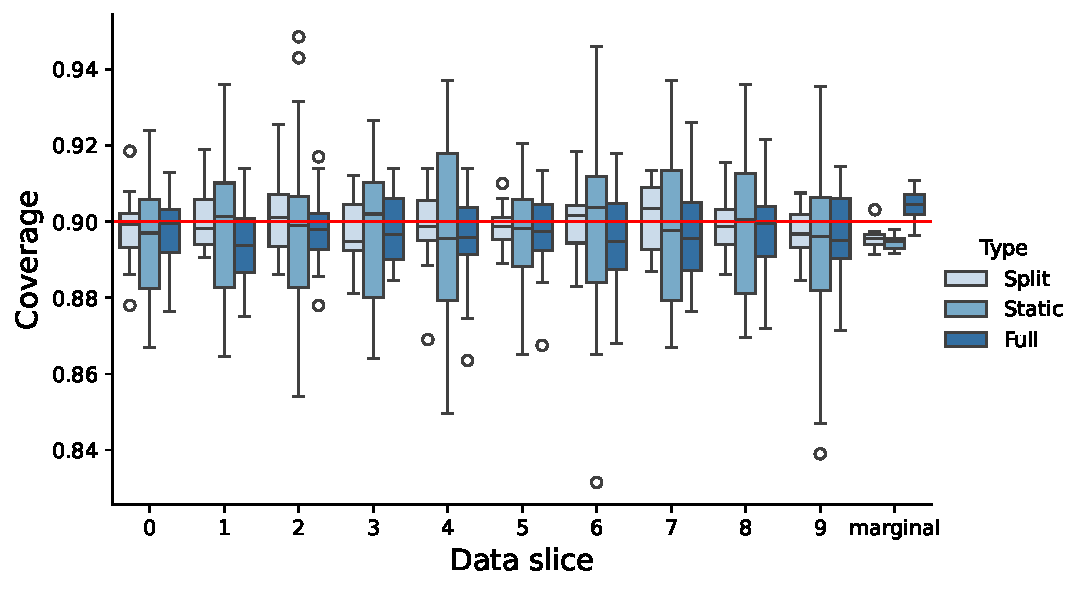
\includegraphics[width=\columnwidth]{Images/random_directions_experiment}
      \end{minipage} &
      \hspace{-1cm}
      \begin{minipage}{.28\columnwidth}
        \caption{\label{fig:random-directions} Coverage of full conformal, split
          conformal, and static split conformal methods on random 20\%
          ``slices'' of CIFAR-100 data.}
      \end{minipage}
    \end{tabular}
  \end{center}
\end{figure}

\section{Conclusion and discussion}

The results in our experiments, though they are relatively small scale,
appear to be consistent with other experiments we do not present for
brevity.
%
In brief: split conformal methods with confidence sets using adaptive
thresholds of the form $\what{C}(x) = \{y \mid \scoreval(x, y) \le
\what{h}(x)\}$ can indeed provide stronger coverage than non-adaptive
thresholds.
%
Moreover, they are \emph{much} faster to compute with than full conformal
methods---in the experiment in Figure~\ref{fig:random-directions},
the split conformal method was roughly 8000$\times$ faster than
the full conformal method.
%
Additionally, they enjoy strong sample-conditional stability
as well as minimax optimality.

In spite of this, when the adaptive threshold
$\what{h}(x)$ comes from a class of functions that is high-dimensional
relative to the size of the data available for calibration,
these methods can undercover, as they exhibit downard bias in their
coverage.
%
This bias is easy to correct for a static threshold
$\what{C}(x) = \{y \mid \scoreval(x, y) \le \what{\tau}\}$ by
simply using a slightly larger quantile, however, it is
unclear how to address it in adaptive scenarios.
%
This makes obtaining a data-adaptive way to compute the coverage bias,
either marginally or along various splits of the validation data,
substantially interesting and a natural direction for future work.
%
Identifying such an offline correction without relying on asymptotic error
calculations, as our heuristic development in
Appendix~\ref{sec:further-simulations} does, could make these procedures
substantially more practical, by both enjoying the test-time speed of split
conformal methods and the coverage accuracy of full-conformal procedures.

\bibliography{bib}
\bibliographystyle{abbrvnat}

\newpage

\appendix

\section{Sample conditional coverage revisited: proofs}
\label{sec:revisiting-conditional-coverage}

As mentioned in Section~\ref{sec:main-basic-sample-coverage},
Proposition~\ref{proposition:sample-conditional-basic} provides a natural point of
departure for developing more sophisticated coverage guarantees.
%
We thus provide this elementary proof, then
demonstrate the result using uniform convergence techniques.
%
These uniform convergence guarantees---which form the basis
for providing guarantees for approximate weighted coverage
(Definition~\ref{definition:weighted-coverage}) also
provide a two-sided bound on sample-conditional coverage:
\begin{corollary}
  \label{corollary:distinct-scores}
  Assume the scores $\scorerv_i = \scoreval(X_i, Y_i)$ are distinct with
  probability 1.
  %
  Then for any $\gamma > 0$, with probability at least
  $1 - 2 e^{-2n \gamma^2}$ over the sample $P_n$,
  \begin{equation*}
    1 - \alpha - \gamma
    \le \P(Y_{n + 1} \in \what{C}_n(X_{n + 1}) \mid P_n)
    \le 1 - \alpha + \frac{1}{n} + \gamma.
  \end{equation*}
\end{corollary}



\subsection{An elementary proof of
  Proposition~\ref{proposition:sample-conditional-basic}}

For the scalar random variable $\scorerv$, define the $\beta$-quantile
\begin{equation}
  \label{eqn:actual-quantile-mapping}
  q\opt(\beta) \defeq \inf \left\{t \in \R
  \mid \P(\scorerv \le t) \ge \beta \right\}.
\end{equation}
Because the CDF is right continuous, we have $\P(S \le q\opt(\beta)) \ge
\beta$, and $\P(S > q\opt(\beta)) = 1 - \P(S \le q\opt(\beta)) \le 1 -
\beta$.
%
For $\gamma > 0$ and any $\tau \in \R$, the inequality
\begin{equation*}
  \P(\scorerv_{n + 1} > \tau) > \alpha + \gamma,
  ~~ \mbox{i.e.} ~~
  \P(\scorerv_{n + 1} \le \tau) < 1 - \alpha - \gamma,
\end{equation*}
implies that $\tau < q\opt(1 - \alpha - \gamma)$.

Consider the event that $\what{\tau}_n < q\opt(1 - \alpha - \gamma)$.
%
For this to occur, it must be the case that
\begin{equation}
  \label{eqn:quantile-too-small}
  \frac{1}{n} \sum_{i = 1}^n \indic{\scorerv_i < q\opt(1 - \alpha - \gamma)}
  \ge 1 - \alpha.
\end{equation}
But this event is unlikely: define the Bernoulli indicator variables $B_i =
\indic{\scorerv_i < q\opt(1 - \alpha - \gamma)}$.
%
Then $\E[B_i] \le 1 -
\alpha - \gamma$, and Hoeffding's inequality implies
that $\wb{B}_n = \frac{1}{n} \sum_{i = 1}^n B_i$ satisfies
\begin{align*}
  \P\left(P_n(\scorerv < q\opt(1 - \alpha - \gamma)) \ge 1 - \alpha
  \right)
  & = \P\left(\wb{B}_n \ge 1 - \alpha\right) \\
  %% & = \P\left(\wb{B}_n - \E[B_1] \ge 1 - \alpha - \E[B_1]\right)
  & \le \P\left(\wb{B}_n - \E[\wb{B}_n] \ge \gamma\right)
  \le \exp(-2 n \gamma^2).
\end{align*}
That is,
\begin{align*}
  \P\left(\what{\tau}_n < q\opt(1 - \alpha - \gamma)\right)
  \le \exp\left(-2n\gamma^2 \right)
\end{align*}
for any $\gamma > 0$, and so we must have
\begin{equation*}
  \P\left(\scorerv_{n + 1} > \what{\tau}_n \mid P_n \right) \le \alpha + \gamma
  ~~ \mbox{with~probability~at~least}~
  1 - e^{-2n\gamma^2}.
\end{equation*}
Rearranging and recalling that $Y_{n + 1} \not \in \what{C}_n(X_{n + 1})$ if
and only if $\scoreval(X_{n+1}, Y_{n + 1}) > \what{\tau}_n$, i.e., if
$\scorerv_{n + 1} > \what{\tau}_n$ gives the result.

\subsection{A proof of Proposition~\ref{proposition:sample-conditional-basic}
  using uniform convergence}
\label{sec:baby-uniform-convergence}

Our alternative approach to the proof of
Proposition~\ref{proposition:sample-conditional-basic} uses
the bounded differences inequality and a uniform concentration
guarantee.
%
First, for any estimated threshold $\what{\tau}_n$, we have
the trivial inequality
\begin{align*}
  \P(\scorerv_{n + 1} > \what{\tau}_n \mid P_n)
  & = \P(\scorerv_{n + 1} > \what{\tau}_n \mid P_n)
  - P_n(\scorerv > \what{\tau}_n)
  + P_n(\scorerv > \what{\tau}_n) \\
  & \le \sup_{\tau \in \R}
  \left|P(\scorerv > \tau)
  - P_n(\scorerv > \tau)\right|
  + P_n(\scorerv > \what{\tau}_n).
\end{align*}
Then because we choose $\what{\tau}_n$ so that
$P_n(\scorerv \le \what{\tau}_n) \ge 1 - \alpha$, we obtain
\begin{subequations}
  \label{eqn:one-VC-simple-deviation}
  \begin{equation}
    \P(\scorerv_{n + 1} > \what{\tau}_n \mid P_n)
    \le \alpha + \sup_{\tau \in \R}
    \left|P(\scorerv > \tau) - P_n(\scorerv > \tau)\right|.
  \end{equation}
  If the values $\scorerv_i$ are distinct, then $P_n(\scorerv \le
  \what{\tau}_n) \le 1 - \alpha + \frac{1}{n}$, and so a completely similar
  calculation yields
  \begin{equation}
    \P(\scorerv_{n + 1} > \what{\tau}_n \mid P_n)
    \ge \alpha - \frac{1}{n} - \sup_{\tau \in \R}
    \left|P(\scorerv > \tau) - P_n(\scorerv > \tau)\right|.
  \end{equation}
\end{subequations}
In either case, if we can control the deviation
$|P(\scorerv > \tau) - P_n(\scorerv > \tau)|$ uniformly across
$\tau$, we will have evidently proved the desired result.

We consider two arguments, the first yielding sharper constants,
while the second generalizes to weighted
coverage.
%
For the first, we apply the Dvoretsky-Kiefer-Wolfowitz
inequality~\cite{Massart90}:
\begin{equation*}
  \P\left(\sup_{\tau \in \R} |P(\scorerv > \tau) - P_n(\scorerv > \tau)|
  \ge t \right) \le 2 e^{-2n t^2}
\end{equation*}
for all $t \ge 0$.
%
Combining the equations~\eqref{eqn:one-VC-simple-deviation}, we
thus obtain that
\begin{align*}
  \P(\scorerv_{n + 1} > \what{\tau}_n \mid P_n)
  \le \alpha + \gamma
  ~~ \mbox{with probability at least}~
  1 - 2 e^{-2 n \gamma^2}.
\end{align*}
If the scores are distinct, the corresponding lower
bound is immediate, giving Corollary~\ref{corollary:distinct-scores}.

The final alternative argument to control the uniform deviations
in the bounds~\eqref{eqn:one-VC-simple-deviation} underpins
our more sophisticated guarantees in the sequel,
relying on uniform concentration guarantees and the
Vapnik-Chervonenkis (VC) dimension.
%
First, recall the classical bounded differences
inequality~\cite{McDiarmid89, Wainwright19}, where we say a function $f :
\mc{X}^n \to \R$ satisfies $c_i$-bounded differences if
\begin{equation*}
  |f(x_1^{i-1}, x_i, x_i, x_{i + 1}^n)
  - f(x_1^{i-1}, x_i', x_{i+1}^n)|
  \le c_i
  ~~ \mbox{for~all~} x_1^{i-1}, x_{i+1}^n,
  x_i, x_i' \in \mc{X}.
\end{equation*}
\begin{lemma}[Bounded differences]
  \label{lemma:bounded-differences}
  Let $X_1, \ldots, X_n$ be independent random variables
  and $f$ satisfy $c_i$-bounded differences. Then
  for all $t \ge 0$,
  \begin{equation*}
    \max\left\{
    \P(f(X_1^n) - \E[f(X_1^n)] \ge t),
    \P(f(X_1^n) - \E[f(X_1^n)] \le -t)
    \right\}
    \le \exp\left(-\frac{2 t^2}{\sum_{i = 1}^n c_i^2}\right).
  \end{equation*}
\end{lemma}

We then observe that $f(P_n) \defeq \sup_{\tau \in \R} |P(\scorerv > \tau) -
P_n(\scorerv > \tau)|$ trivially satisfies bounded differences.
%
Indeed, let $P_n'$ differ from $P_n$ in a single observation.
%
Then
defining $\linf{P - P_n} = \sup_\tau |P(\scorerv > \tau)
- P_n(\scorerv > \tau)|$ for shorthand, we obtain
\begin{align*}
  \left|\linf{P - P_n} - \linf{P - P_n'}\right|
%%   \lefteqn{\sup_{\tau \in \R}
%%     |P(\scorerv > \tau) - P_n(\scorerv > \tau)|
%%     - \sup_{\tau \in \R}
%%     |P(\scorerv > \tau) - P_n'(\scorerv > \tau)|} \\
  & \le
  \linf{P_n - P_n'}
  \le \frac{1}{n}
%%   \sup_{\tau \in \R}
%%   \left\{|P(\scorerv > \tau) - P_n(\scorerv > \tau)|
%%   -
%%   |P(\scorerv > \tau) - P_n'(\scorerv > \tau)|\right\}
%%   \le \sup_{\tau \in \R}
%%   |P_n(\scorerv > \tau) - P_n'(\scorerv > \tau)|
%%   \le \frac{1}{n}
\end{align*}
by the triangle inequality and that only one example may change.
%
Lemma~\ref{lemma:bounded-differences} then implies
\begin{align*}
  \P\left(\linf{P - P_n} \ge \E[\linf{P - P_n}]
  + t \right) \le e^{-2nt^2}
\end{align*}
for $t \ge 0$, so that we need only control $\E[\linf{P - P_n}]$.
%
For this, we perform a standard symmetrization
argument~\cite[e.g.][Ch.~2.3]{VanDerVaartWe96}: let $P_n^0 = \frac{1}{n}
\sum_{i = 1}^n \varepsilon_i \pointmass_{\scorerv_i}$, where $\varepsilon_i
\simiid \uniform\{\pm 1\}$ are i.i.d.\ Rademacher variables
and $\pointmass_{\scorerv_i}$ denotes a point mass on $\scorerv_i$.
%
By introducing independent copies of $\scorerv_i$
and applying Jensen's inequality~\cite[Lemma 2.3.1]{VanDerVaartWe96},
we have the bound
\begin{equation*}
  \E\left[\linf{P_n - P}\right]
  \le 2 \E\left[\linf{P_n^0}\right]
  = 2 \E\left[\sup_{\tau \in \R} \bigg|\frac{1}{n}
    \sum_{i = 1}^n \varepsilon_i \indic{\scorerv_i > \tau}
    \bigg|\right].
\end{equation*}
Because the class of functions $\scoreval \mapsto \indic{\scoreval > \tau}$
has VC-dimension at most 1, Dudley's entropy
integral (see, e.g.~\cite[Corollary 2.2.8 and Thm.~2.6.7]{VanDerVaartWe96}
or~\cite[Eq.~(5.5.1)]{Wainwright19}) shows that
\begin{equation*}
  \E\left[\linf{P_n^0}\right]
  \le \frac{c}{\sqrt{n}}
\end{equation*}
for a numerical constant $c$.
%
We then obtain that for any $\gamma \ge 0$,
\begin{align*}
  \P\left(\scorerv_{n + 1} > \what{\tau}_n \mid P_n\right)
  \le \alpha + \frac{c}{\sqrt{n}} + \gamma
  ~~ \mbox{w.p.}~
  1 - e^{-2n \gamma^2}
\end{align*}
by the inequalities~\eqref{eqn:one-VC-simple-deviation}, where
$c$ is a numerical constant.

\subsection{Proof of Proposition~\ref{proposition:distinct-scores}}
\label{sec:proof-distinct-scores}

%% $P(S > \what{\tau}_n) > \alpha + \gamma$
%% if and only if
%% $P(S \le \what{\tau}_n) < 1 - \alpha - \gamma$
%% if and only if
%% $\what{\tau}_n < q\opt(1 - \alpha - \gamma)$.
%% That is, there is $t$ such that
%% $t < q\opt(1 - \alpha - \gamma)$ and for which
%% $P_n(S \le t) \ge 1 - \alpha$.

Recall the quantile mapping $q\opt$ from
the definition~\eqref{eqn:actual-quantile-mapping} and that
for fixed $\gamma \in [0, \alpha]$, the event
$\what{\tau}_n < q\opt(1 - \alpha - \gamma)$
can occur only if
$P_n(\scorerv < q\opt(1 - \alpha - \gamma)) \ge 1 - \alpha$.
%
Then defining $B_i = \indic{\scorerv_i < q\opt(1 - \alpha - \gamma)}$
and recalling inequality~\eqref{eqn:quantile-too-small},
we obtain
\begin{align*}
  \P(\what{\tau}_n < q\opt(1 - \alpha - \gamma))
  \le \P(\wb{B}_n \ge 1 - \alpha)
  = \P(\wb{B}_n - \E[\wb{B}_n] \ge 1 - \alpha - \E[\wb{B}_n]).
\end{align*}
Define $p(\gamma) = \E[B_i]
= \P(\scorerv < q\opt(1 - \alpha - \gamma)) < 1 - \alpha - \gamma$,
so that $t = t(\gamma) \defeq 1 - \alpha - p(\gamma) > \gamma$.
%
Then $\var(B_i) = p(\gamma)(1 - p(\gamma))
= (\alpha + t)(1 - \alpha - t)$, and Bernstein's inequality
implies
\begin{align*}
  \P(\wb{B}_n - \E[\wb{B}_n] \ge t)
  & \le \exp\left(-\frac{n t^2}{2 (1 - \alpha - t) (\alpha + t)
    + \frac{2}{3} t}\right) \\
  & = \exp\left(-\frac{n t^2}{2 (1 - \alpha) \alpha +
    (\frac{8}{3} - 4 \alpha) t - t^2}\right)
  \le \exp\left(-\frac{n t^2}{2(1 - \alpha) \alpha
    + \frac{8}{3} t}\right).
\end{align*}
Notably, $t \mapsto \frac{nt^2}{2(1 - \alpha) \alpha + \frac{8}{3} t}$
is increasing in $t$, so that
\begin{equation*}
  \P(\what{\tau}_n < q\opt(1 - \alpha - \gamma))
  \le \exp\left(-\frac{n \gamma^2}{2(1 - \alpha) \alpha + \frac{8}{3} \gamma}
  \right).
\end{equation*}


If the scores $\scorerv$ have a density,
$\P(\scorerv \le q\opt(\beta)) = \beta$ for any $\beta \in (0, 1)$.
%
Then we may also consider the event that $\what{\tau}_n > q\opt(1 - \alpha +
\gamma)$.
%
For this to occur, we require
\begin{equation*}
  P_n(\scorerv < q\opt(1 - \alpha + \gamma)) \le 1 - \alpha,
\end{equation*}
and defining $B_i = \indic{\scorerv_i < q\opt(1 - \alpha + \gamma)}$,
we have $\E[B_i] = 1 - \alpha + \gamma$ and so
\begin{align*}
  \P(\wb{B}_n \le 1 - \alpha)
  = \P(\wb{B}_n - \E[\wb{B}_n] \le -\gamma)
  & \le \exp\left(-\frac{n \gamma^2}{2 (1 - \alpha + \gamma)
    (\alpha - \gamma) + \frac{2}{3} \gamma}\right) \\
  & \le \exp\left(-\frac{n \gamma^2}{2 (1 - \alpha)\alpha + \frac{2}{3}
    \gamma}\right)
\end{align*}
for $\gamma \in [0, \alpha]$.
%
Combining the two cases, for $\gamma \ge 0$ we have
\begin{equation*}
  \max\left\{\P\left(\what{\tau}_n < q\opt(1 - \alpha - \gamma)\right),
  \P\left(\what{\tau}_n > q\opt(1 + \alpha + \gamma)\right)\right\}
%%   \what{\tau}_n \not \in
%%     [q\opt(1 - \alpha - \gamma),
%%       q\opt(1 + \alpha + \gamma)]\right)
  \le \exp\left(-\frac{n \gamma^2}{2\alpha(1 - \alpha) + \frac{8}{3}
    \gamma}\right).
\end{equation*}
Solving to guarantee the right hand side is at most $\delta$ yields
\begin{equation*}
  \gamma_n \defeq \frac{4 \log \frac{1}{\delta}}{3n}
  + \sqrt{\left(\frac{4}{3 n} \log \frac{1}{\delta}\right)^2 +
    \frac{2 \alpha(1 - \alpha)}{n}
    \log \frac{1}{\delta}}.
\end{equation*}
Applying a union bound implies
Proposition~\ref{proposition:distinct-scores}.


%% It remains, therefore, to control the fluctuations of the process
%% \begin{equation*}
%%   \frac{1}{n} \sum_{i = 1}^n \phi(X_i) \indic{\scorerv_i < \theta^\top
%%     \phi(X_i)}
%% \end{equation*}
%% as $\theta$ varies; once we can do this, we will have the result.
%% %


%% Theorem~\ref{theorem:approximate-conditional-coverage} now follows.
%% %
%% In particular, we take $\mc{H} = \{h(x) = \<\theta, \phi(x)\>\}_{\theta \in
%%   \R^d}$, which has VC-dimension $d$, and
%% recognize that $Y_{n + 1} \in \what{C}_n(X_{n + 1})$ if and only if
%% $\scorerv_{n + 1} = \scoreval(X_{n + 1}, Y_{n + 1}) \le \what{h}(X_{n + 1})$.

%% Via a minor extension, we obtain the following corollary
%% of the proposition.
%% \begin{corollary}
%%   \label{corollary:high-prob-deviation}
%%   Let $\mc{H}$ be a class of functions with VC-dimension $k$ and
%%   $\alpha \in [0, 1]$.
%%   Then there exists a numerical constant $c$ such that for $t \ge 0$,
%%   \begin{equation*}
%%     \P\left(\sup_{u \neq 0, h \in \mc{H}}
%%     \frac{1}{\ltwo{u}}
%%     \E_{P_n}
%%     \left[\<u, \phi(X)\>
%%       \left(\indic{\scorerv < h(X)} - (1 - \alpha)\right)\right]
%%     \ge
%%     c \radphi \left(\sqrt{\frac{k \log \frac{n}{k}}{n}}
%%     + t \right)\right) \le e^{-nt^2}.
%%   \end{equation*}
%% \end{corollary}

\section{Proof of Theorems~\ref{theorem:one-sided-sharp}
  and~\ref{theorem:two-sided-sharp}}
\label{sec:proof-sharp}

We split the proof into three sections, first giving the shsared
building blocks, then specializing.

\subsection{Proof of Theorems~\ref{theorem:one-sided-sharp}
  and~\ref{theorem:two-sided-sharp}: building blocks}
\label{sec:proof-sharp-building-blocks}

Our proof leverages a combination of Talagrand's concentration inequalities
for empirical processes, a VC-dimension calculation, and localized
Rademacher complexities~\cite{BartlettBoMe05, Koltchinskii06a}.
We begin with the form of Talagrand's empirical
process inequality with constants due to \citet{Bousquet02thesis}.

\begin{lemma}[Talagrand's empirical process inequality]
  \label{lemma:talagrand}
  Let $\mc{F}$ be a countable class of functions with
  $Pf = 0$ and $\linf{f} \le b$ for $f \in \mc{F}$. Let $Z = \sup_{f \in \mc{F}}
  P_n f$ and $\sigma^2 = \sigma^2(\mc{F}) = \sup_{f \in \mc{F}} Pf^2$.
  Define $v^2 \defeq \sigma^2 + 2b \E[Z]$.
  Then for $t \ge 0$,
  \begin{equation*}
    \P\left(Z \ge \E[Z] + \sqrt{2 v^2 t} + b\frac{t}{3}\right)
    \le e^{-nt}.
  \end{equation*}
\end{lemma}

Because we will consider functions of the form $f(x, \scoreval) = \<u,
\phi(x)\> \indic{\<\theta, \phi(x)\> > \scoreval}$, we also require
some control over the complexity of such rank-one-like products.
\begin{lemma}
  \label{lemma:product-vc}
  Let $\mc{H}$ and $\mc{G}$ be classes of functions with
  VC-dimensions $d_1$ and $d_2$, respectively. Then
  the classes of functions
  \begin{equation*}
    \mc{F} \defeq \{f \mid f(x) = g(x) \indic{h(x) > 0}\}
    ~~ \mbox{and} ~~
    \mc{F}_+ \defeq \{f \mid f(x) = g(x) \indic{h(x) > 0} - c g(x)\}
  \end{equation*}
  where $c$ is a constant
  have VC-dimension $O(1)(d_1 + d_2)$.
\end{lemma}
\begin{proof}
  For a set of points $x_1, \ldots, x_n$, let $\mc{S}(x_1^n, \mc{H}) =
  \{\indic{h(x_i) > 0}\}_{i = 1}^n$ be the set of ``sign'' vectors that $h$
  realizes.
  %
  By definition of the VC-dimension and the Sauer-Shelah lemma, this set has
  cardinality at most $\sum_{i = 0}^{d_1} \binom{n}{i} \le
  (\frac{ne}{d_1})^{d_1}$.
  %
  Similarly, the set of signs
  \begin{equation*}
    \mc{S}(x_1^n, \mc{F})
    = \{\sign(g(x_i)) \cdot \indic{h(x_i) > 0}\}_{i = 1}^n
  \end{equation*}
  has cardinality at most $\sum_{i = 0}^{d_1} \binom{n}{i} \cdot \sum_{i =
    0}^{d_2} \binom{n}{i} \le (\frac{ne}{d_1})^{d_1}
  (\frac{ne}{d_2})^{d_2}$.
  %
  If $n$ is large enough that
  \begin{equation*}
    \left(\frac{ne}{d_1}\right)^{d_1} \cdot \left(\frac{ne}{d_2}\right)^{d_2}
    < 2^n,
  \end{equation*}
  then certainly $\mc{F}$ cannot shatter $n$ points; this occurs
  once $n \ge c \cdot (d_1 + d_2)$ for some numerical constant $c$.
  %
  For the second class the argument is similar.
\end{proof}

\newcommand{\rademacher}{\mathfrak{R}}

For the next lemma, our main technical building block for convergence, we
consider the class of functions $\mc{F}$ indexed by $u \in \ball$ and $h \in
\mc{H}$, where $\mc{H}$ is a class with VC-dimension at most $d$,
with
\begin{equation}
  \label{eqn:product-function-class}
  f(x, \scoreval) = f_{u,h}(x, \scoreval)
  \defeq \<u, \phi(x)\> \indic{\scoreval > h(x)}.
\end{equation}
Each of these functions evidently satisfies
$|f(x, \scoreval)| \le \radphi$.
%
The variance proxy
\begin{equation}
  \label{eqn:variance-proxy}
  v^2(u, h) \defeq v^2(f_{u,h}) = P f_{u, h}(X, \scorerv)^2
  = \E[\<\phi(X), u\>^2 \indic{\scorerv > h(X)}]
\end{equation}
and its empirical variant
\begin{equation*}
  v_n^2(u, h) = P_n f_{u,h}(X, \scorerv)^2
  = \frac{1}{n} \sum_{i = 1}^n \<\phi(X_i), u\>^2 \indic{\scorerv_i > h(X_i)}.
\end{equation*}
will allow us to bound deviations of $P_n f$ from $P f$ relative
to $v^2(f)$.

For later use, we
recall the \emph{empirical Rademacher complexity} of a function class
$\mc{F}$,
\begin{equation*}
  \rademacher_n(\mc{F})
  \defeq \frac{1}{n} \E\left[\sup_{f \in \mc{F}}
    \sum_{i = 1}^n \varepsilon_i f(X_i) \mid X_1^n\right],
\end{equation*}
where $\varepsilon_i \simiid \uniform\{\pm 1\}$ are random signs.
%
In some cases, we will require \emph{localized Rademacher
complexities}~\cite{BartlettBoMe05, Koltchinskii06a} around
a class $\mc{F}_r \defeq \{f \mid Pf^2 \le r^2\}$, which
contains functions of small variance, allowing us to ``relativize''
bounds.
%
\citet[Proof of Corollary 3.7]{BartlettBoMe05} demonstrate the following.
\begin{lemma}
  Let $\mc{F}$ be a star-convex collection of functions,
  meaning that $f \in \mc{F}$ implies $\lambda f \in \mc{F}$
  for $\lambda \in [0, 1]$, and assume that $\sup_x |f(x)| \le b$
  and $\mc{F}$ has VC-dimension $d$. Then
  \begin{equation}
    \label{eqn:rademacher-vc-control}
    \E\left[\rademacher_n(\mc{F}_r)\right]
    \le \frac{\radphi}{n} + 
    c r \sqrt{\frac{d}{n} \log\frac{\radphi}{r}}
    ~~ \mbox{if}~~
    r^2 > \radphi^2 \frac{d}{n} \log \frac{n}{d},
  \end{equation}
  where $c < \infty$ is a numerical constant.  
\end{lemma}


We will combine the VC-bound in Lemma~\ref{lemma:product-vc},
the version of
Talagrand's empirical process inequality in Lemma~\ref{lemma:talagrand}, and
a localization argument on Rademacher complexities
via inequality~\eqref{eqn:rademacher-vc-control}
to prove the following lemma in Appendix~\ref{sec:proof-peel-your-potatoes}.
\begin{lemma}
  \label{lemma:peel-your-potatoes}
  Let $\mc{F}$ be the class of functions~\eqref{eqn:product-function-class}.
  Let $K_n = 1 + \log_2 n$. Then
  for all $t \ge 0$, with probability at least
  $1 - K_n e^{-t}$ over the draw of the sample $P_n$,
  \begin{equation*}
    |(P_n - P) f|
    \le c \left[v(f) \sqrt{\frac{d \log n + t}{n}}
    + \radphi \frac{d \log n + t}{n}\right]
  \end{equation*}
  simultaneously for all $f \in \mc{F}$, where $c < \infty$ is a numerical
  constant.
  In addition, with the same probability,
  \begin{equation*}
    \left|(P_n - P)\<u, \phi(X)\>\right|
    \le c \left[\sqrt{P \<u, \phi\>^2}
      \sqrt{\frac{d \log n + t}{n}}
      + \radphi \frac{d \log n + t}{n}
      \right]
  \end{equation*}
  simultaneously for all $u \in \ball$.
\end{lemma}

Next we present a version of a result appearing as \cite[Theorem
  14.12]{Wainwright19} (the result there assumes functions are mean-zero,
but an inspection of the proof shows this is unnecessary); see also the
results of \cite{Mendelson14} and~\cite[Proof of Proposition
  1]{DuchiRu18a}. These show that second moments satisfy one-sided
concentration bounds with high probability as soon as
we have the fourth moment condition
\begin{equation}
  \label{eqn:four-moments}
  \E[f^4(X, \scorerv)] \le b^2 \E[f^2(X, \scorerv)]
  ~~ \mbox{for~all~} f \in \mc{F}.
\end{equation}
For the setting we consider, where $\mc{F}$ consists
of product functions~\eqref{eqn:product-function-class},
inequality~\eqref{eqn:four-moments} immediately
holds with $b = \radphi$, though tighter constants may be possible.
\begin{lemma}
  \label{lemma:no-concentration-lower}
  There exist numerical constants $0 < c$ and $C < \infty$ such that
  the following holds. Let inequality~\eqref{eqn:four-moments} hold and
  for $\mc{F}_r = \{f \mid Pf^2 \le r^2\}$, let
  $r$ satisfy $\E[\rademacher_n(\mc{F}_r)] \le \frac{r^2}{C b}$. Then
  with probability at least $1 - e^{-c n r^2 / b^2}$,
  \begin{equation*}
    P_n f^2 \ge \half P f^2
    ~~ \mbox{simultaneously~for~all~} f
    ~ \mbox{s.t.}~ v(f) \ge r.
  \end{equation*}
\end{lemma}

Inequality~\eqref{eqn:rademacher-vc-control} shows the conclusions of
of Lemma~\ref{lemma:no-concentration-lower} hold if the radius $r$
satisfies
\begin{equation*}
  r \sqrt{\frac{d}{n} \log \frac{n}{d}}
  \lesssim \frac{r^2}{\radphi}
  ~~ \mbox{or} ~~
  r^2 \gtrsim \radphi^2 \cdot \frac{d}{n} \log \frac{n}{d}.
\end{equation*}
We then obtain the following consequence:
\begin{lemma}
  \label{lemma:specialize-no-concentration}
  Let $r^2 \gtrsim \radphi^2 \frac{d}{n} \log \frac{n}{d}$.
  %%  and define
  %%   \begin{equation*}
  %%     \mc{H}_r \defeq \left\{h \in \mc{H} \mid
  %%     \mbox{there exists}~ u \in \ball
  %%     ~ \mbox{s.t.} ~ P \<u, \phi(X)\>^2 \indic{\scorerv > h(X)}
  %%     \ge r^2 \right\}.
  %%   \end{equation*}
  Then with probability at least $1 - e^{-c n r^2 / \radphi^2}$,
  \begin{equation*}
    P_n\<u, \phi(X)\>^2 \indic{\scorerv > h(X)}
    \ge \half P\<u, \phi(X)\>^2 \indic{\scorerv > h(X)}
  \end{equation*}
  simultaneously over $u \in \ball$ and $h$ such that
  $P\<u, \phi(X)\>^2 \indic{\scorerv > h(X)} \ge r^2$.
\end{lemma}

Now, let $\what{h} = \<\what{\theta}, \phi(\cdot)\>$, where $\what{\theta}$
solves the problem~\eqref{eqn:empirical-quantile-estimator}.
%
Then simultaneously for all $u \in \ball$,
with probability at least $1 - K_n e^{-t}$,
\begin{equation}
  \label{eqn:bart-ride}
  \left|(P_n - P)\<u, \phi(X)\> \indic{\scorerv > \what{h}(X)}\right|
  \le c \left[v(\what{h}, u)
    \sqrt{\frac{d \log n + t}{n}}
    + \radphi \frac{d \log n + t}{n}\right]
\end{equation}
by Lemma~\ref{lemma:peel-your-potatoes}.
Moreover, for $r^2 \gtrsim \radphi^2 \frac{d}{n} \log \frac{n}{d}$,
either $v(\what{h}, u) \le r$ or
\begin{equation*}
  v^2(\what{h}, u)
  \le 2 P_n \<\phi(X), u\>^2 \indic{\scorerv > \what{h}(X)}
\end{equation*}
by Lemma~\ref{lemma:specialize-no-concentration} (with the appropriate
probability $1 - e^{-cr^2 / \radphi^2}$).

\subsection{Proof of Theorem~\ref{theorem:one-sided-sharp}: nonnegative
  weights}
\label{sec:proof-one-sided-sharp}

We now specialize our development to the particular
cases that $\<u, \phi(x)\> \ge 0$ for all $x \in
\mc{X}$.
%
First, we leverage the particular structure of the quantile
loss to give a non-probabilistic bound on the empirical
weights.
\begin{lemma}
  \label{lemma:one-directional-coverageish}
  Let $u$ be such that $\<u, \phi(x)\> \ge 0$ for all $x \in \mc{X}$.
  Then
  \begin{equation*}
    P_n \<\phi(X), u\> \indic{\scorerv > \what{h}(X)}
    \le \alpha P_n \<\phi(X), u\>.
  \end{equation*}
  If additionally $\scorerv_i$ are all distinct, then
  \begin{equation*}
    P_n \<\phi(X), u\> \indic{\scorerv > \what{h}(X)}
    \ge \alpha P_n \<\phi(X), u\> - \radphi(u) \frac{d}{n}.
  \end{equation*}
\end{lemma}
\begin{proof}
  The directional derivative
  $\loss'_\alpha(t; 1) \defeq \lim_{\delta \downarrow 0}
  \frac{\loss_\alpha(t + \delta) - \loss_\alpha(t)}{\delta}
  = \indic{t \ge 0} - (1 - \alpha)$.
  Then
  \begin{align*}
    P_n \<\phi(X), u\> \indic{\scorerv > \what{h}(X)}
    & = P_n\<\phi(X), u\>
    \left(1 - \alpha
    - \indic{\scorerv \le \what{h}(X)}\right)
    + P_n \<u, \phi(X)\> \alpha \\
    & = 
    P_n \<\phi(X), u\>
    \left(-\loss'_\alpha(\what{h}(X) - \scorerv; 1)\right)
    + \alpha P_n\<u, \phi(X)\>.
  \end{align*}
  Letting $L_n(h) = P_n \loss_\alpha(h(X) - \scorerv)$, we now use that
  directional derivatives are positively homogeneous~\cite{HiriartUrrutyLe93}
  and that by assumption $\what{h}$ minimizes
  $P_n \loss_\alpha(h(X) - \scorerv)$ over
  functions of the form $h(x) = \<\theta, \phi(x)\>$ to obtain
  \begin{equation*}
    P_n \<\phi(X), u\>
    \left(-\loss'_\alpha(\what{h}(X) - \scorerv; 1)\right)
    = - P_n\loss'_\alpha(\what{h}(X) - \scorerv; \<\phi(X), u\>)
    = - L_n'(\what{h}(X); u).
  \end{equation*}
  But of course, as $\what{h}$ minimizes $L_n$,
  we have $L_n'(\what{h}(X); u) \ge 0$ for all $u$, and so
  \begin{equation*}
    P_n\<\phi(X), u\> \indic{\scorerv > \what{h}(X)}
    \le \alpha P_n \<u, \phi(X)\>.
  \end{equation*}

  If $\scorerv_i$ are all distinct, then considering the
  left directional derivative, we also have
  \begin{align*}
    P_n\<\phi(X), u\> \indic{\scorerv \ge \what{h}(X)} \ge
    \alpha P_n \<u, \phi(X)\>.
  \end{align*}
  If $\mc{I}_0 = \{i \mid \what{h}(X_i) = \scorerv_i\}$,
  then $\card(\mc{I}_0) \le d$, and so
  \begin{equation*}
    0 \ge P_n \<\phi(X), u\>
    \left(\indic{\scorerv > \what{h}(X)}
    - \indic{\scorerv \ge \what{h}(X)}\right)
    = -P_n \<\phi(X), u\> \indic{\scorerv = \what{h}(X)}
    \ge -\radphi(u) \frac{d}{n}.
  \end{equation*}
  Rearranging and performing a bit of algebra, we
  obtain the second claim of the lemma.
\end{proof}

From the lemma, we see that
\begin{align}
  \lefteqn{
    P \<u, \phi(X)\> \left(\indic{\scorerv > \what{h}(X)}
    - \alpha\right)} \nonumber \\
  & = (P - P_n)\<u, \phi(X)\> \left(\indic{\scorerv > \what{h}(X)}
  - \alpha\right)
  + P_n \<u, \phi(X)\> \left(\indic{\scorerv > \what{h}(X)}
  - \alpha\right) \nonumber \\
  & \le (P - P_n) \<u, \phi(X)\> \indic{\scorerv > \what{h}(X)}
  - \alpha (P - P_n) \<u, \phi(X)\>
  \label{eqn:incorporate-the-alpha}
\end{align}
by Lemma~\ref{lemma:one-directional-coverageish}.
%
Additionally, the lemma implies that
\begin{align*}
  P_n\<\phi(X), u\>^2 \indic{\scorerv > \what{h}(X)}
  & \le \radphi(u) P_n \<\phi(X), u\> \indic{\scorerv > \what{h}(X)}
  \le \radphi(u) \alpha P_n \<\phi(X), u\>.
\end{align*}
We use this to control the first term in the
expansion~\eqref{eqn:incorporate-the-alpha}
by combining these bounds with inequality~\eqref{eqn:bart-ride}
and considering
that $v(\what{h}, u) \le r$ or $v(\what{h}, u) > r$
where $r^2 = O(1) \radphi^2 \frac{d}{n} \log \frac{n}{d}$.
%
In the latter, we have
$v^2(\what{h}, u) \le c \radphi(u) \alpha P_n\<\phi(X), u\>$.
%
We have therefore shown that for
any $r^2 \gtrsim \frac{d}{n} \log \frac{n}{d}$,
with probability at
least $1 - K_n e^{-t} - e^{-n r^2}$,
for all $u \in \ball$
with $\<u, \phi(x)\> \ge 0$,
\begin{align}
  \label{eqn:ashby-stop}
  \lefteqn{\left|(P_n - P)\<u, \phi(X)\> \indic{\scorerv > \what{h}(X)}
    \right|}
  \\
  & \le c \left[
    \left(\sqrt{\radphi(u) \alpha P_n \<u, \phi(X)\>} + \radphi r\right)
    \sqrt{\frac{d \log n + t}{n}}
    + \radphi \frac{d \log n + t}{n}
    \right].
  \nonumber
\end{align}

Applying Lemma~\ref{lemma:peel-your-potatoes} to the quantity
$P_n\<u, \phi(X)\>$ shows that simultaneously
for all $u \in \ball$,
\begin{align*}
  |(P_n - P)\<u, \phi(X)\>| & \le
  c
  \left[\sqrt{\radphi(u) P\<u, \phi(X)\>}
    \sqrt{\frac{d \log n + t}{n}}
    + \radphi \frac{d \log n + t}{n}\right]
\end{align*}
with probability at least $1 - K_n e^{-t}$.
%
Substituting this into the
bounds~\eqref{eqn:incorporate-the-alpha} and~\eqref{eqn:ashby-stop}, and
ignoring lower-order terms (because $\alpha \le 1$), we obtain the guarantee
that for all $t \ge 0$ and $r^2 \gtrsim \frac{d}{n} \log \frac{n}{d}$, then
with probability at least $1 - 2 K_n e^{-t} - e^{-n r^2}$, for all $u$ such
that $P\<u, \phi(X)\> \ge \radphi \frac{d \log n + t}{n}$,
\begin{align*}
  \E\left[
    \<u, \phi(X)\> \left(\indic{\scorerv > \what{h}(X)} - \alpha\right)
    \mid P_n\right]
  & \le
  c \left[
    \left(\sqrt{\alpha \radphi(u) P\<u, \phi(X)\>} + \radphi r\right)
    \sqrt{\frac{d \log n + t}{n}}
    + \radphi \frac{d \log n + t}{n}
    \right]
\end{align*}
and for all $u$ such that $P\<u, \phi(X)\> \le \radphi
\frac{d \log n + t}{n}$,
\begin{align*}
  \E\left[
    \<u, \phi(X)\> \left(\indic{\scorerv > \what{h}(X)} - \alpha\right)
    \mid P_n\right]
  \le c \radphi \left[r \sqrt{\frac{d \log n + t}{n}}
    + \frac{d \log n + t}{n}\right].
\end{align*}
Combining the inequalities and replacing
$r^2$ with $\frac{d \log n + t}{n}$
gives the first claim of Theorem~\ref{theorem:one-sided-sharp}.

For the second claim, when the scores $\scorerv_i$ are distinct,
note simply that we may replace
inequality~\eqref{eqn:incorporate-the-alpha}
with
\begin{align*}
  \lefteqn{
    P \<u, \phi(X)\> \left(\indic{\scorerv > \what{h}(X)}
    - \alpha\right)} \nonumber \\
  & = (P - P_n)\<u, \phi(X)\> \left(\indic{\scorerv > \what{h}(X)}
  - \alpha\right)
  + P_n \<u, \phi(X)\> \left(\indic{\scorerv > \what{h}(X)}
  - \alpha\right) \nonumber \\
  & \ge (P - P_n) \<u, \phi(X)\> \indic{\scorerv > \what{h}(X)}
  - \alpha (P - P_n) \<u, \phi(X)\>
  - \radphi(u) \frac{d}{n}.
\end{align*}
The remainder of the argument is, \emph{mutatis mutandis}, identical to the
proof of the first claim of the theorem.

\subsection{Proof of Theorem~\ref{theorem:two-sided-sharp}: distinct scores}
\label{sec:proof-two-sided-sharp}

Because of the distinctness of
$\scorerv_i$ and that we assume $\phi_1(x) = 1$ (that is, we include
the constant offset), the optimality conditions for
the quantile loss imply that
\begin{equation*}
  \frac{d}{n} \ge \sum_{i = 1}^n \indic{\scorerv_i > \what{h}(X_i)}
  - \alpha \ge -\frac{d}{n}.
\end{equation*}
So if $\radphi(u) \defeq \sup_{x \in \mc{X}} |\<u, \phi(x)\>|$, then
\begin{equation*}
  P_n\<\phi(X), u\>^2 \indic{\scorerv > \what{h}(X)}
  \le \radphi^2(u) \left(\alpha  + \frac{d}{n} \right).
\end{equation*}
Applying inequality~\eqref{eqn:bart-ride},
we find that with probability at least $1 - K_n e^{-t} - e^{-c n r^2 /
  \radphi^2}$,
\begin{equation*}
  \left|(P_n - P)\<u, \phi(X)\> \indic{\scorerv > \what{h}(X)}\right|
  \le c \left[\left(\radphi(u)\sqrt{\alpha}
    + r\right)\sqrt{\frac{d \log n + t}{n}}
    + \radphi  \frac{d \log n + t}{n}\right].
\end{equation*}
The deviations $\alpha (P_n - P)\<u, \phi(X)\>$ are of smaller
order than this by Lemma~\ref{lemma:peel-your-potatoes}.


%% For an empirical measure $P_n$ on points $Z_1, \ldots, Z_n$, define $P_n^0
%% = \frac{1}{n} \sum_{i = 1}^n \varepsilon_i \pointmass_{Z_i}$ and
%% the empirical Rademacher complexity
%% \begin{equation*}
%%   \rademacher_n(\mc{F}) \defeq \rademacher_n(\mc{F} \mid P_n)
%%   \defeq \E\left[\sup_{f \in \mc{F}} P_n^0 f \mid P_n \right].
%% \end{equation*}

%% \begin{lemma}
%%   Let
%% \end{lemma}
%% \begin{proof}
%%   Let $\mc{N}_\epsilon$ be an $\epsilon$-cover of $\ball_2$ of minimal
%%   cardinality, so that $\log \card(\mc{N}_\epsilon ) \lesssim
%%   d \log \frac{1}{\epsilon}$. Then
%%   for each $v \in \ball_2$, there exists $v^0 \in \mc{N}_\epsilon$
%%   with $\ltwo{v - v^0} \le \epsilon$, while
%%   \begin{align*}
%%     \<v, P_n \phi(X) \indic{\scorerv > h(X)}\>
%%     & = \<v - v^0, P_n \phi(X) \indic{\scorerv > h(X)}\>
%%     + \<v^0, P_n \phi(X) \indic{\scorerv > h(X)}\> \\
%%     & \in \<v^0, P_n \phi(X) \indic{\scorerv > h(X)}\>
%%     \pm \epsilon \radphi.
%%   \end{align*}
%%   For any $f \in \mc{F}_r$, where $f(x, \scoreval) = \<v, \phi(x)\>
%%   \indic{\scoreval > h(x)}$, there exists $v^0 \in \mc{N}_\epsilon$ such
%%   that $|f(x, \scoreval) - \<v^0, \phi(x)\> \indic{\scoreval > h(x)}| \le
%%   \epsilon \radphi$. So
%%   \begin{align*}
%%     \rademacher_n(\mc{F}_r)
%%     & = \E\left[\sup_{v \in \ball_2}
%%       \sup_{h \in \mc{H}_r} \<v, P_n^0 \phi(X) \indic{\scorerv > h(X)}\>\right] \\
%%     & \le \epsilon \radphi
%%     + \E\left[\max_{v \in \mc{N}_\epsilon}
%%       \sup_{h \in \mc{H}_r}
%%       \left\<v, P_n^0 \phi(X) \indic{\scorerv > h(X)}\right\>\right]
%%   \end{align*}
%% \end{proof}

%% Let $\psi$ be any sub-root function satisfying
%% \begin{equation*}
%%   \psi(r) \ge \E\left[\rademacher_n(\mc{F}_r)\right]
%% \end{equation*}
%% for $r \ge r\opt$. Now, if $r \ge \psi(r)$, then \cite[Corollary
%%   2.2]{BartlettBoMe05} gives that with probability at least $1 - 1/n$,
%% \begin{equation*}
%%   \{f \in \mc{F} \mid Pf^2 \le r^2\}
%%   \subset \{f \in \mc{F} \mid P_n f^2 \le 2 r^2 \}
%% \end{equation*}
%% so
%% \begin{

\section{Technical proofs}

\subsection{Proof of Lemma~\ref{lemma:bound-deviation-ltwo}}
\label{sec:proof-bound-deviation-ltwo}

When $\ball_2$ is the $\ell_2$-ball,
\begin{equation*}
  \E\left[\sup_{h \in \mc{H}, u \in \ball_2}
    \<u, Z_n(h) - \E[Z_n(h)]\>\right]
  = \E\left[\sup_{h \in \mc{H}} \ltwo{Z_n(h) - \E[Z_n(h)]}
    \right].
\end{equation*}
Performing a typical symmetrization argument, we let $P_n^0 = \frac{1}{n}
\sum_{i = 1}^n \varepsilon_i \pointmass_{X_i, \scorerv_i}$ be the
symmetrized empirical measure, where $\varepsilon_i \simiid \uniform\{\pm
1\}$ are i.i.d.\ Rademacher variables, and define the symmetrized process
$Z_n^0(h) = \frac{1}{n} \sum_{i = 1}^n \varepsilon_i \phi(X_i)
\indic{\scorerv_i > h(X_i)}$.
%
Then for the (random) set of vectors
$\mc{V}_n = \{(\indic{\scorerv_1 > h(X_1)}, \ldots, \indic{\scorerv_n >
  h(X_n)})\}_{h \in \mc{H}} \subset \{0, 1\}^n$
\begin{align*}
  \E\left[\sup_{h \in \mc{H}} \ltwo{Z_n(h) - \E[Z_n(h)]} \right]
  & \le 2 \E\left[\sup_{h \in \mc{H}} \ltwo{Z_n^0(h)}\right]
  \le 2 \E\left[\max_{v \in \mc{V}_n}
    \ltwobigg{\frac{1}{n} \sum_{i = 1}^n \varepsilon_i \phi(X_i) v_i}\right].
\end{align*}
Now, we recognize that because the vectors $\phi$ lie in a Hilbert
space,
we enjoy certain dimension free concentration guarantees.
%
In particular, we have for any fixed $v \in \{0, 1\}^n$ that
\begin{equation*}
  \P\left(\ltwobigg{\sum_{i = 1}^n \varepsilon_i \phi(X_i) v_i} \ge t
  \mid X_1^n \right)
  \le 2 \exp\left(-\frac{t^2}{2 \Phi_n^2}\right),
\end{equation*}
where $\Phi_n^2 \defeq \sum_{i = 1}^n \ltwo{\phi(X_i)}^2$ by
\citet[Theorem 3.5]{Pinelis94} (see also~\cite[Corollary
  10]{HowardRaMcSe20}).
%
In particular, using that for $U$ a nonnegative random variable
$\E[U] = \int_0^\infty \P(U \ge u) du$,
we obtain
\begin{align*}
  \E\left[\max_{v \in \mc{V}_n} \ltwobigg{\sum_{i = 1}^n
      \varepsilon_i \phi(X_i) v_i}
    \mid X_1^n \right]
  & \le \int_0^\infty \P
  \left(\max_{v \in \mc{V}_n}
  \ltwobigg{\sum_{i = 1}^n
    \varepsilon_i \phi(X_i) v_i} \ge t \mid X_1^n \right) dt \\
  & \le t_0
  + 2 \card(\mc{V}_n) \int_{t_0}^\infty
  \exp\left(-\frac{t^2}{2 \Phi_n^2}\right) dt.
\end{align*}
Recognizing the Gaussian tail bound
that
\begin{equation*}
  \int_c^\infty e^{-\frac{t^2}{2 \sigma^2}} dt
  = \sqrt{2 \pi \sigma^2}
  \int_{c/\sigma}^\infty \frac{1}{\sqrt{2\pi}} e^{-z^2 / 2} dz
  \le \sqrt{2 \pi \sigma^2}
  \min\left\{\frac{1}{\sqrt{2\pi}}
  \frac{\sigma}{c}, 1 \right\}
  \exp\left(-\frac{c^2}{2\sigma^2}\right)
\end{equation*}
by Mills' ratio, we see that for any $t_0 \ge 0$,
\begin{align*}
  \E\left[\max_{v \in \mc{V}_n} \ltwobigg{\sum_{i = 1}^n
      \varepsilon_i \phi(X_i) v_i}
    \mid X_1^n \right]
  & \le t_0 + 2 \card(\mc{V}_n)
  \cdot \frac{\Phi_n^2}{t_0}
  \exp\left(-\frac{t_0^2}{2 \Phi_n^2}\right).
\end{align*}

Finally, recognize that $\mc{V}_n$ has cardinality at most $(\frac{e
  n}{k})^{k}$ by the Sauer-Shelah lemma because $\mc{H}$ has VC-dimension
$k$.
%
Consequently, we may take $t_0^2 = 2 \log \card(\mc{V}_n) \Phi_n^2$ to
obtain the bound
\begin{align*}
  \E\left[\max_{v \in \mc{V}_n} \ltwobigg{\sum_{i = 1}^n
      \varepsilon_i \phi(X_i) v_i}
    \mid X_1^n \right]
  & \le \sqrt{2 \log \card(\mc{V}_n)} \Phi_n
  + \frac{\Phi_n}{\sqrt{2 \log \card(\mc{V}_n)}}
  \le 2 \sqrt{k \log \frac{n e}{k}} \cdot \Phi_n.
\end{align*}
Take expectations over $X_1^n$.

\subsection{Proof of Lemma~\ref{lemma:peel-your-potatoes}}
\label{sec:proof-peel-your-potatoes}

For $r \ge 0$, define the localized class
\begin{equation*}
%%   \mc{F}_r \defeq \left\{f \in \mid f(x, \scoreval)
%%   = \<v, \phi(x)\> \indic{\scoreval > h(x)}
%%   ~ \mbox{for~some}~ h \in \mc{H}_r \right\}.
  \mc{F}_r \defeq
  \left\{f \in \mc{F}
  \mid Pf^2 = \E[\<v, \phi(X)\>^2 \indic{\scorerv
      > h(X)}] \le r^2 \right\}.
\end{equation*}
Note that $\mc{F}_r$ always includes the 0 function and is star-convex,
because if $f \in \mc{F}_r$, then $\lambda f \in \mc{F}_r$ for $\lambda \in
[0, 1]$.
%
Recalling inequality~\eqref{eqn:rademacher-vc-control},
the second term dominates the first, and so
\begin{equation*}
  \E\left[\rademacher_n(\mc{F}_r)\right]
  \le c r \sqrt{\frac{d}{n} \log \frac{n}{d}}
  ~~ \mbox{if}~~
  r^2 \ge \radphi^2 \frac{d}{n} \log \frac{n}{d}.
\end{equation*}

Define the random variable $Z_n(r) \defeq
\sup_{f \in \mc{F}_r} (P_n - P) f = \sup_{f \in \mc{F}_r} |(P_n - P) f|$, the
equality following by symmetry of $\mc{F}_r$. Then
Talagrand's concentration inequality (Lemma~\ref{lemma:talagrand}) implies
that
\begin{equation*}
  \P\left(Z_n(r) \ge \E[Z_n(r)]
  + \sqrt{2 (r^2 + 2 \radphi \E[Z_n(r)]) t}
  + \frac{\radphi}{3} t \right) \le e^{-nt}
\end{equation*}
for all $t \ge 0$.  Applying a standard symmetrization argument and
inequality~\eqref{eqn:rademacher-vc-control},
we thus obtain that for $r^2 \ge \radphi^2 \frac{d}{n} \log \frac{n}{d}$,
with probability at least $1 - e^{-t}$,
\begin{equation*}
  Z_n(r) \le c r \sqrt{\frac{d \log n}{n}}
  + c \sqrt{\frac{r^2}{n^2} + \frac{\radphi^2}{n}
    r \sqrt{\frac{d \log n}{n}}} \sqrt{t}
  + \frac{\radphi t}{3n}.
\end{equation*}
As the last step, we apply a peeling
argument~\cite{Wainwright19, vandeGeer00}: consider the intervals
\begin{equation*}
  E_k \defeq \openleft{2^{k-1}\frac{\radphi^2 d \log n}{n}}{
    2^k \frac{\radphi^2 d \log n}{n}}
  ~~
  k = 1, 2, \ldots, K_n \defeq \ceil{\log_2 \frac{n}{d \log n}}.
\end{equation*}
Let $\mc{F}^k = \{f \in \mc{F} \mid  Pf^2 \in E_k\}$,
where $\mc{F}^0 = \{f \in \mc{F} \mid Pf^2 \le \frac{d \log n}{n}\}$. Then
evidently $\cup_{k = 0}^{K_n} \mc{F}^k = \mc{F}$, and letting
$r_k^2 = 2^k \radphi^2 \frac{d \log n}{n}$, we have
$\mc{F}_{r_k} \subset \mc{F}^k$. So by a union bound,
with probability at least $1 - (K_n + 1)e^{-t}$,
\begin{subequations}
  \label{eqn:peeling-inequalities}
  \begin{equation}
    Z_n(r_k) \le c r_k \sqrt{\frac{d \log n}{n}} + c
    \sqrt{\frac{r_k^2}{n^2} + \frac{\radphi}{n}
      \sqrt{\frac{r_k^2 d \log n}{n}}} \sqrt{t} + \frac{\radphi}{3n} t
    ~~ \mbox{for~} k = 1, \ldots, K_n
  \end{equation}
  and
  \begin{equation}
    Z_n(r_0) \le c \frac{d \log n}{n}
    + \sqrt{\frac{r_0^2}{n^2} + \frac{\radphi}{n}
      \frac{d \log n}{n}} \sqrt{t} + \frac{\radphi t}{3n}.
  \end{equation}
\end{subequations}

Recall the definition $v^2(f) \defeq Pf^2 = \var(f) + (Pf)^2$. Then
$f \in \mc{F}^k$ implies $\half r_k \le v(f) \le r_k$, so that
on the event that all the inequalities~\eqref{eqn:peeling-inequalities}
hold, then simultaneously for all $f$ satisfying
$v^2(f) \ge \frac{d \log n}{n}$, then
\begin{equation*}
  \left|(P_n - P) f\right|
  \le c v(f) \sqrt{\frac{d \log n}{n}}
  + c \sqrt{\frac{v^2(f)}{n^2}
    + \frac{\radphi}{n} \sqrt{v^2(f) \frac{d \log n}{n}}}
  \sqrt{t} + \frac{\radphi}{3n} t,
\end{equation*}
while for all $f$ with $v^2(f) \le \frac{d \log n}{n}$ we have
\begin{equation*}
  |(P_n - P) f|
  \le c \frac{d \log n}{n}
  + c \sqrt{\frac{d \log n}{n^3}
    + \frac{\radphi}{n} \frac{d \log n}{n}} \sqrt{t} + \frac{\radphi}{3n} t.
\end{equation*}
(To obtain the absolute bounds, we have used that $f \in \mc{F}$ implies
$-f \in \mc{F}$ and each set $\mc{F}_r$ and $\mc{F}^k$ is symmetric.)
Finally, we note that
\begin{align*}
  \sqrt{\frac{v^2(f)}{n^2}
    + \frac{\radphi}{n}
    \sqrt{v^2(f) \frac{d \log n}{n}}}
  & \le \sqrt{\frac{v^2(f)}{n^2}
    + \frac{\radphi^2 d \log n}{2 n^2}
    + \frac{v^2(f)}{2 n}} \\
  & \le \frac{\radphi \sqrt{d \log n}}{\sqrt{2} n}
  + \frac{v(f)}{\sqrt{n}},
\end{align*}
which implies the first statement of Lemma~\ref{lemma:peel-your-potatoes}.

The second statement follows via the same argument.

\section{Further simulations}
\label{sec:further-simulations}

We can incorporate a few recent theoretical results to enhance
the practical performance of the proposed conformalization procedures,
allowing some additional performance gains, while simultaneously
exhibiting the need for future work.
%
We consider mostly the difference between the full conformal approach that
\citet{GibbsChCa23} develop and the split-conformal approaches
that simply minimize the empirical
loss~\eqref{eqn:empirical-quantile-estimator}.
%
Our theoretical results provide no guidance to lower-order corrections
to the desired level $\alpha$ to guarantee (exact) marginal coverage
rather than approximate sample-conditional coverage, and
so we proceed a bit heuristically here, using theoretical
results to motivate modifications of the level $\alpha$ that
do not change the sample-conditional coverage results we provide, but
which turn out to be empirically effective.

\newcommand{\alphadesired}{\alpha_{\textup{des}}}

To motivate our tweaks, recall the classical (unconditional) conformal
approach to achieve exact finite-sample marginal coverage $\P(Y_{n + 1} \in
\what{C}_n(X_{n + 1}))$, where the confidence confidence set $\what{C}_n(x)
= \{y \mid \scoreval(x, y) \le \what{\tau}_n\}$.
%
Setting $\what{\tau}_n = \quant_{(1 + 1/n) (1 - \alpha)}(\scorerv_1^n)$, the
slightly enlarged quantile, guarantees $(1 - \alpha)$ coverage; this follows
by letting $\scorerv_{(i,n)}$ be the order statistics of $\scorerv_1^n$ and
$\scorerv_{(i, n + 1)}$ those of $\scorerv_1^{n + 1}$, and noting that the
score $\scorerv_{n + 1} \le \scorerv_{(k,n)}$ if and only if $\scorerv_{n +
  1} \le \scorerv_{(k , n + 1)}$~\cite[Lemma 2]{RomanoPaCa19}, so the
inflation by $\frac{n+1}{n}$ is necessary.
%
Equivalently, if we wish to achieve coverage $(1 - \alphadesired)$ using the
estimator~\eqref{eqn:empirical-quantile-estimator} with feature mapping
$\phi(x) = 1$ fit at level $\alpha$, then $\alpha$ must solve $(1 - \alpha)
= (1 + \frac{1}{n}) (1 - \alphadesired)$, that is, $\alpha = 1 - (1 +
\frac{1}{n})(1 - \alphadesired) = (1 + \frac{1}{n}) \alphadesired -
\frac{1}{n}$.
%
That is, quantile regression under-covers.

When $\phi : \mc{X} \to \R^d$, it is then natural to heuristically imagine
that the order statistics ought to ``swap orders'' by at most roughly $d$
items and so we ought to target coverage $\frac{n + d}{n}(1 -
\alphadesired)$; unfortunately, it escapes our ability to prove such a
result currently.
%
Nonetheless, we consider a ``naive'' adaptation of the confidence level,
setting $\alpha$ to solve
\begin{equation}
  \label{eqn:naive-alpha}
  (1 - \alpha) = \left(1 + \frac{d}{n}\right) (1 - \alphadesired),
  ~~ \mbox{or} ~~
  \alpha = \left(1 + \frac{d}{n}\right) \alphadesired - \frac{d}{n},
\end{equation}
and then choosing $\what{\theta}$ to
minimize~\eqref{eqn:empirical-quantile-estimator} with this $\alpha$,
which we term the ``naive'' choice.
%
\citet{BaiMeWaXi21} give an alternative perspective, where they show
that the actual marginal coverage achieved by quantile regression
at level $\alpha$ in the high-dimensional scaling $d, n \to \infty$ with
$d/n \to \kappa \in (0, 1)$ is
\begin{equation*}
  (1 - \alpha) - \frac{d}{n} \left(\half - \alpha\right) + o(d/n)
\end{equation*}
for $\alpha < \half$, at least when the covariates are Gaussian.
%
Solving this and ignoring the higher-order term, we recognize that to
achieve desired coverage $\alpha$, we ought (according to this heuristic) to
compute the estimator~\eqref{eqn:empirical-quantile-estimator} using
$\alpha$ solving
\begin{equation}
  \label{eqn:bai-alpha}
  (1 - \alphadesired) = (1 - \alpha) - \frac{d}{n}
  \left(\half - \alpha\right)
  %% = 1 - \left(1 - \frac{d}{n}\right) \alpha - \frac{d}{2n},
  ~~ \mbox{or} ~~
  \alpha = \frac{\alphadesired - \frac{d}{2n}}{1 - \frac{d}{n}}.
\end{equation}
We call the choice~\eqref{eqn:bai-alpha} the ``scaling'' choice.
%
Neither of the rescalings~\eqref{eqn:naive-alpha} or~\eqref{eqn:bai-alpha}
have any effect on the convergence guarantees our theory provides, as they
are of lower order.

We perform two synthetic experiments that give a
sense of the coverage properties of the methods we have analyzed.
%
These exploratory experiments help provide justification for the heuristic
corrections to the desired level $\alpha$ we set in the real data
experiments.

\subsection{Level rescaling on a simple synthetic dataset}

%% CODE FOR THIS: Code/basic_conditional_coverage.py

\newcommand{\noise}{\varepsilon}

For our first experiment, we consider the simple setting of
a standard Gaussian linear model, where we observe
\begin{equation*}
  y_i = \<w\opt, x_i\> + \noise_i,
  ~~ \noise_i \simiid \normal(0, 1)
  ~~ \mbox{and} ~~ x_i \simiid \normal(0, I_d).
\end{equation*}
We mimic the experiment \citet[Fig.~3]{GibbsChCa23} provide,
but we investigate the coverage properties of the
coverage set from the estimator~\eqref{eqn:empirical-quantile-estimator}
with uncorrected $\alpha$ and level $\alpha$ corrected
either naively~\eqref{eqn:naive-alpha} or via the scaling
correction~\eqref{eqn:bai-alpha}.
%
In all cases, we use the feature map $\phi(x) = (1, \indic{x_1 > 0}, \ldots,
\indic{x_d > 0}) \in \{0, 1\}^{d + 1}$ indicating nonnegative coordinates.
%
Figure~\ref{fig:simulation-correction-coverage} displays the results of this
experiment for 1000 trials, where in each trial, we draw $w\opt \sim
\uniform(\sphere^{d-1})$, fit a regression estimator $\what{w}$ on a
training dataset of size $n_{\textup{train}} = 100$ using least squares,
then conformalize this predictor using a validation set of size $n$ and
evaluate its coverage on a test dataset of size $n_{\textup{test}} = 10
n_{\textup{train}} = 1000$.
%
We vary the
ratio $n / d$ of the validation dataset, keeping $d = 20$ fixed.
%
From the figure, it is clear that the uncorrected confidence
set using $\alpha = \alphadesired = .1$
undercovers, especially when the ratio $n/d < 20$ or so.
%
The naive correction~\eqref{eqn:naive-alpha} appears to be a bit
conservative, while the scaling correction~\eqref{eqn:bai-alpha}
is more effective.

\begin{figure}[ht]
  \begin{center}
    \begin{tabular}{cc}
      \hspace{-1cm}
      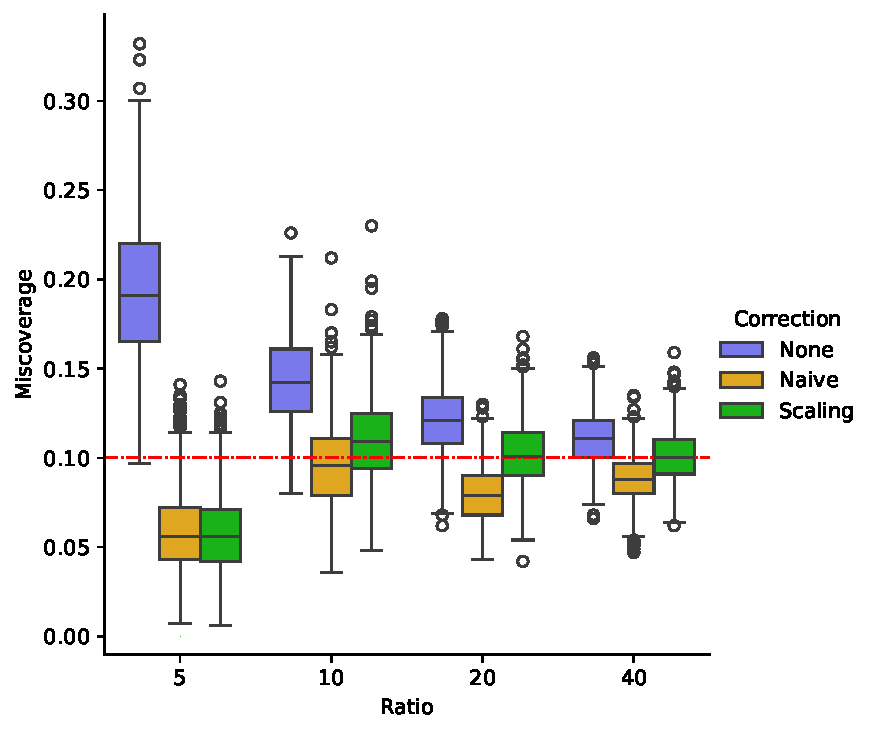
\includegraphics[width=.55\columnwidth]{%
        Images/miscoverage_guassian_linreg} &
      \hspace{-.5cm}
      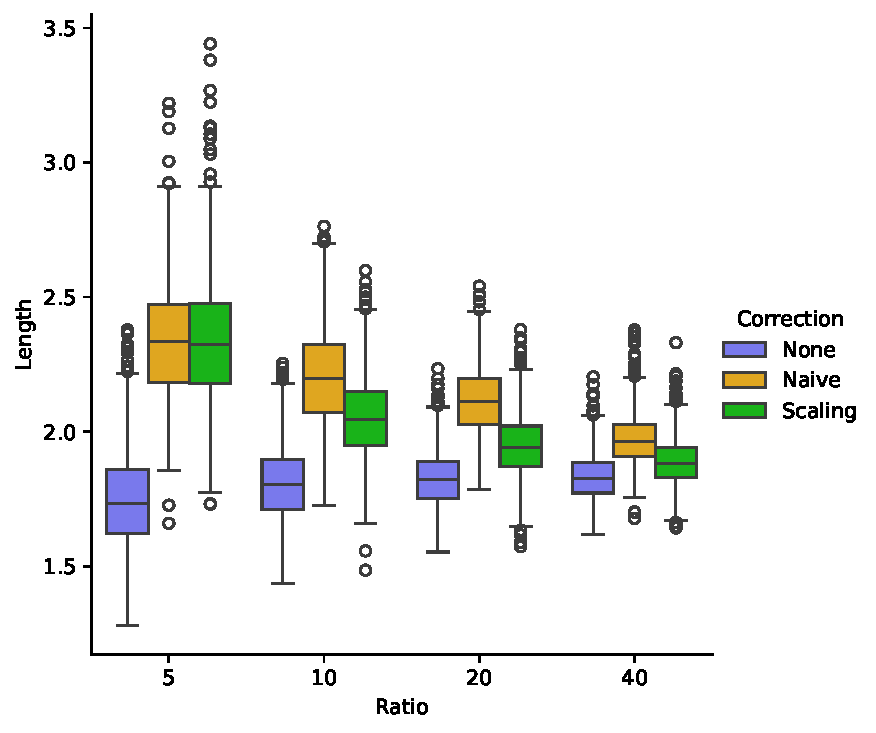
\includegraphics[width=.55\columnwidth]{%
        Images/confsize_guassian_linreg.pdf} \\
      (a) & (b)
    \end{tabular}
    \caption{\label{fig:simulation-correction-coverage} Impact of the
      correction to $\alpha$ used in fitting the conformal
      predictor~\eqref{eqn:empirical-quantile-estimator} for a desired level
      $\alphadesired = .1$, i.e., 90\% coverage. The ``None'' correction
      uses $\alpha = \alphadesired$, ``Naive'' uses the
      correction~\eqref{eqn:naive-alpha}, and ``Scaling'' uses the
      correction~\eqref{eqn:bai-alpha}.  (a) Coverage rates with the desired
      coverage marked as the red line. (b) Width of predictive intervals
      $\what{C}(x) = \{y \in \R \mid |\what{f}(x) - y| \le
      \what{\theta}^\top \phi(x)\}$.}
  \end{center}
\end{figure}

\subsection{Full conformal versus split-conformal predictions}
\label{sec:offline-sin-simulation}

We briefly look at the coverage properties of the full conformalization
method~\eqref{eqn:implicit-full-confidence-set} from the
paper~\citep{GibbsChCa23}, comparing with split-conformal
methods~\eqref{eqn:empirical-quantile-estimator}, on a synthetic regression
dataset we design to have asymmetric mean-zero heteroskedastic noise.
%
We generate pairs $(X_i, Y_i) \in \R^2$ according to
$Y = f(x) + \noise(x)$,
discretizing $x \in [0, 1]$ into bins
$B_i = \{x \mid \frac{i}{k} \le x < \frac{i + 1}{k}\}$,
$i = 0, \ldots, k - 1$, for $k = 5$.
%
Within each experiment, we
draw $U_0, U_1 \simiid \uniform[-1, 1]$ and
$\phi_0, \phi_1 \simiid \uniform[\frac{\pi}{4}, 4 \pi]$
to define
\begin{equation*}
  f(x) = U_0 \cos(\phi_0 \cdot x)
  + U_1 \sin(\phi_1 \cdot x).
\end{equation*}
Within the $i$th region $\frac{i}{k} \le x < \frac{i + 1}{k}$ we
set $\lambda_{0,i} = \exp(3 - \frac{3}{k} i)$ and
$\lambda_{1,i} = \exp(4 - \frac{3}{k} i)$, i.e.,
evenly spaced in $\{e^{3}, \ldots, e^0\}$ and $\{e^{4}, \ldots, e^{1}\}$,
and draw
\begin{equation*}
  \noise(x) \sim \begin{cases} \expdist(\lambda_{0,i})
    & \mbox{with probability}~
    \frac{\lambda_{0,i}}{\lambda_{0,i} + \lambda_{1,i}}
    = \frac{1}{1 + e} \\
    -\expdist(\lambda_{1,i})
    & \mbox{otherwise},
  \end{cases}
\end{equation*}
so that $\E[\noise(x) \mid x] = 0$ but the noise is skewed upward,
with variance increasing in $i$.

Figure~\ref{fig:little-silly-experiment} shows the results of this
experiment over 200 independent trials, where in each
experiment we draw a new mean function $f$ and fit it using
a degree 5 polynomial regression on a training
set of size $n_{\textup{train}} = 200$.
%
The conformalization methods use a group-indicator featurization $\phi(x) =
(1, \indic{x \in B_1}, \ldots, \indic{x \in B_k})$ and confidence sets
$C(x) = \{y \mid \theta_0^\top \phi(x) \le y \le \theta_1^\top
\phi(x)\}$.
%
Within each trial, we compute miscoverage
proportions $\P(Y \not \in \what{C}(X) \mid X \in B_i)$ for each bin $i$ on
a test set of size 500, drawing a new function $f$.
%
We vary the size of the validation data $n_{\textup{val}}
= \{10 k, 20k, 40k, 80k, 160k\}$, and
use the scaling correction~\eqref{eqn:bai-alpha} to set $\alpha$ for
the split-conformal method.
%
The figure plots results for validation sizes $40k$ and $160k$; from the
figure---which is consistent with our other sample sizes and
experiments---we see that when the validation size is large relative to the
dimension of the mapping $\phi$, both methods are similar; for smaller
ratios, the offline method undercovers slightly within the groups, though
its marginal coverage remains near perfect in spite of the very non-Gaussian
data.

\begin{figure}
  \begin{center}
    \begin{tabular}{cc}
      \hspace{-.5cm}
      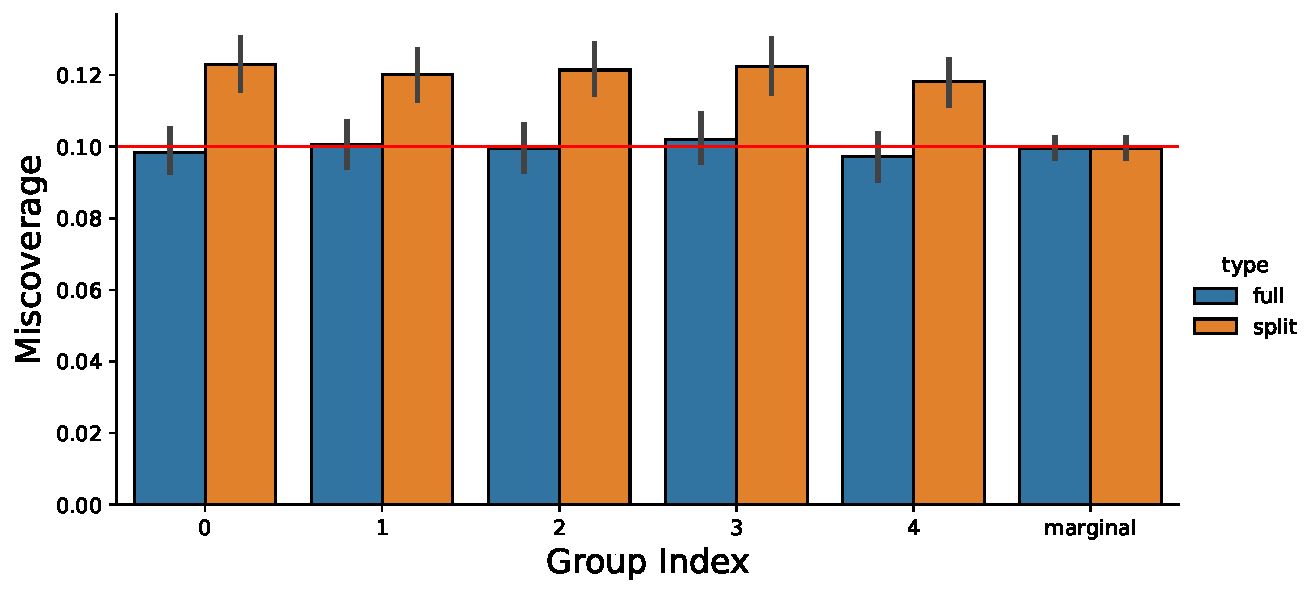
\includegraphics[width=.5\columnwidth]{Images/group_miscoverage_ratio_40}
      &
      \hspace{-.25cm}
      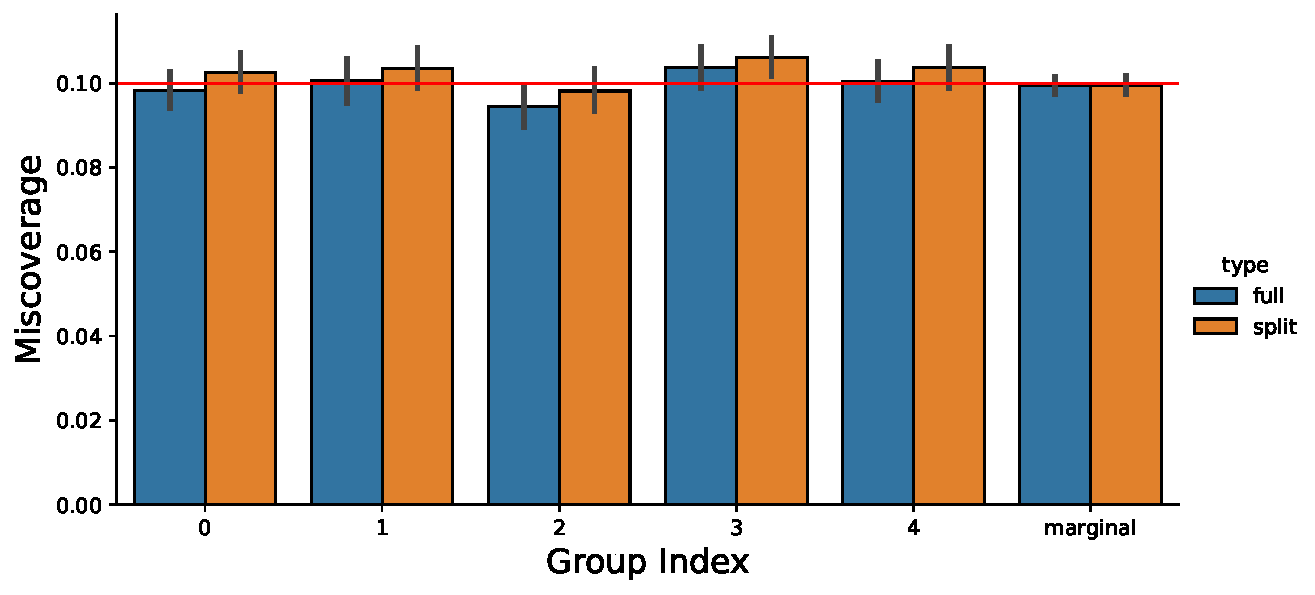
\includegraphics[width=.5\columnwidth]{Images/group_miscoverage_ratio_160} \\
      (a) & (b) \\
      \hspace{-.5cm}
      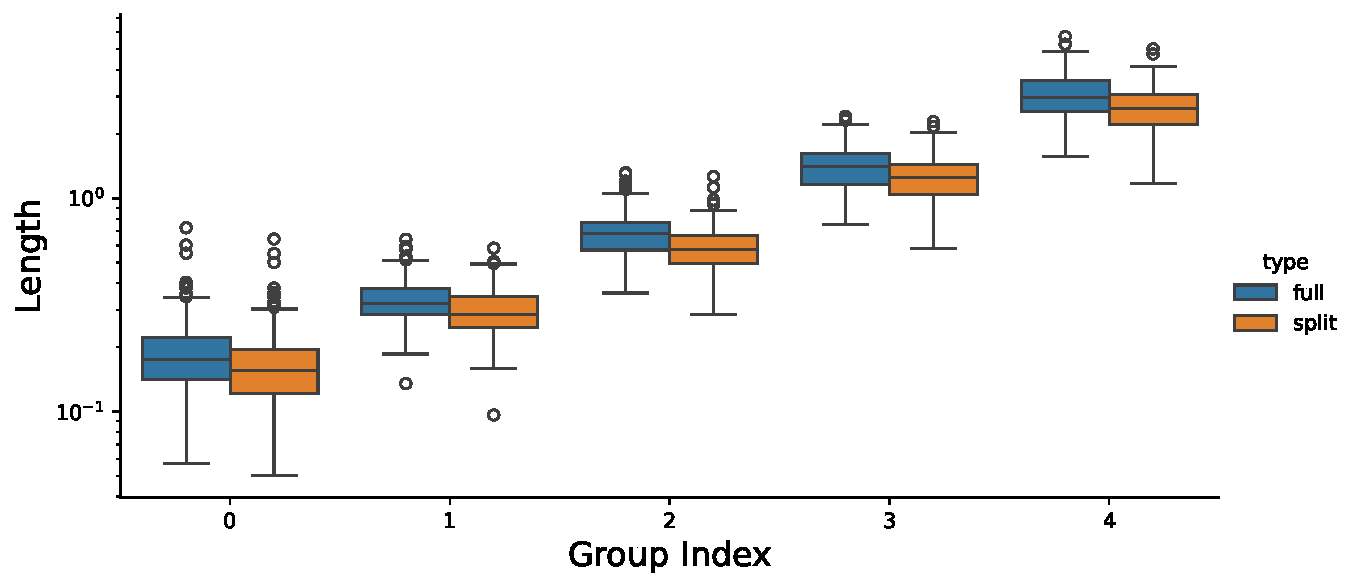
\includegraphics[width=.5\columnwidth]{Images/group_length_ratio_40} &
      \hspace{-.25cm}
      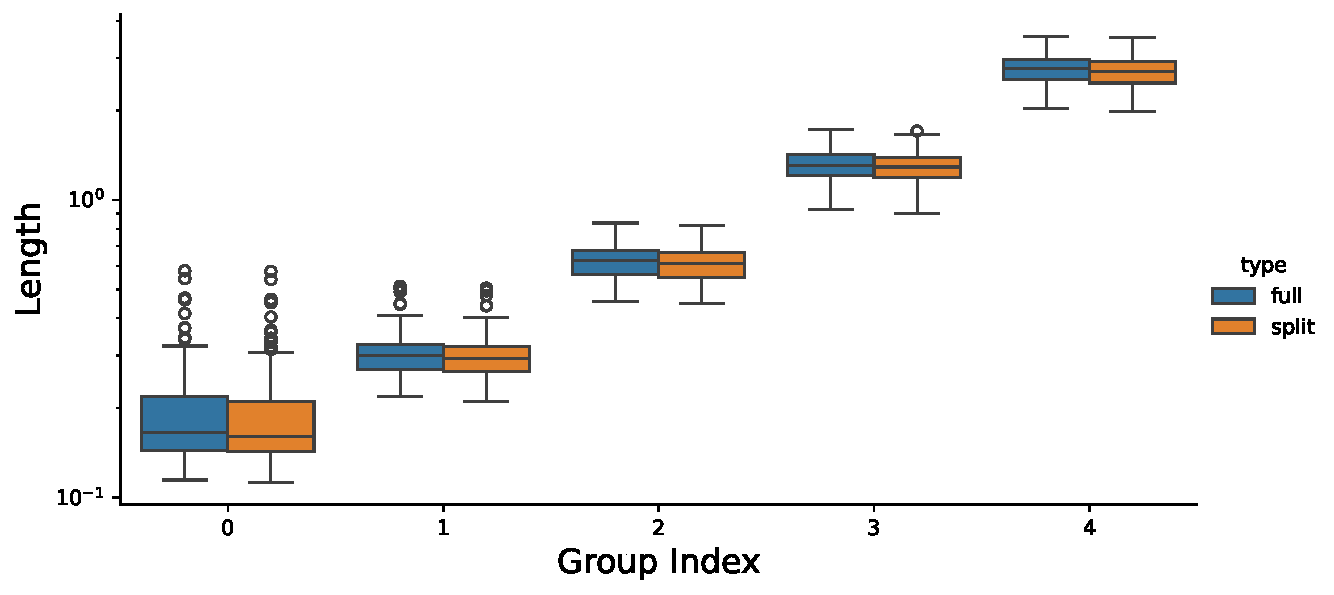
\includegraphics[width=.5\columnwidth]{Images/group_length_ratio_160} \\
      (c) & (d)
    \end{tabular}
    \caption{
      \label{fig:little-silly-experiment}
      Comparison of full- and split-conformal
      methods on the simulated sinusoidal data of
      Sec.~\ref{sec:offline-sin-simulation} with
      $n_{\textup{train}} = 200$ training examples and target
      miscoverage $\alpha = .1$.
      Plots (a) and (c) use validation
      sample sizes $n_{\textup{val}} = 20 k = 100$,
      while (b) and (d) use
      $n_{\textup{val}} = 160 k = 800$. Plots (a) and
      (b) show miscoverage $\P(Y \not \in \what{C}(X) \mid X \in B_i)$ by
      group $B_i$; plots (c) and (d) prediction interval lengths.
%%       For
%%       larger validation sizes, both methods perform similarly;
%%       the offline method has somewhat lower coverage at small validation
%%       sample sizes.
    }
  \end{center}
\end{figure}

We remark in passing that the full conformal method requires roughly $10
\times$ the amount of time to compute predictions as the split conformal
method requires to both fit a quantile prediction model and make its
predictions.
%
Once the split-conformal quantile model is available---it has been
fit---this difference becomes roughly a factor
of 2000--4000 in our experiments.
%
For some applications, this may be immaterial; for others, it may be
a substantial expense, suggesting that a decision between
the offline method and the online procedure may boil down to
one of computational feasibility.

\newpage

\section*{NeurIPS Paper Checklist}

\begin{enumerate}

\item {\bf Claims}
    \item[] Question: Do the main claims made in the abstract and introduction accurately reflect the paper's contributions and scope?
    \item[] Answer: \answerYes{} % Replace by \answerYes{}, \answerNo{}, or \answerNA{}.
    \item[] Justification:
    \item[] Guidelines:
    \begin{itemize}
        \item The answer NA means that the abstract and introduction do not include the claims made in the paper.
        \item The abstract and/or introduction should clearly state the claims made, including the contributions made in the paper and important assumptions and limitations. A No or NA answer to this question will not be perceived well by the reviewers. 
        \item The claims made should match theoretical and experimental results, and reflect how much the results can be expected to generalize to other settings. 
        \item It is fine to include aspirational goals as motivation as long as it is clear that these goals are not attained by the paper. 
    \end{itemize}

\item {\bf Limitations}
    \item[] Question: Does the paper discuss the limitations of the work performed by the authors?
    \item[] Answer: \answerYes{} % Replace by \answerYes{}, \answerNo{}, or \answerNA{}.
    \item[] Justification: The main contributions of the paper are
      theoretical. The main limitation of the paper (see the Discussion
      section) is the theoretical results do not provide exact coverage,
      which appears to be challenging for sample-conditional coverage.
    \item[] Guidelines:
    \begin{itemize}
        \item The answer NA means that the paper has no limitation while the answer No means that the paper has limitations, but those are not discussed in the paper. 
        \item The authors are encouraged to create a separate "Limitations" section in their paper.
        \item The paper should point out any strong assumptions and how robust the results are to violations of these assumptions (e.g., independence assumptions, noiseless settings, model well-specification, asymptotic approximations only holding locally). The authors should reflect on how these assumptions might be violated in practice and what the implications would be.
        \item The authors should reflect on the scope of the claims made, e.g., if the approach was only tested on a few datasets or with a few runs. In general, empirical results often depend on implicit assumptions, which should be articulated.
        \item The authors should reflect on the factors that influence the performance of the approach. For example, a facial recognition algorithm may perform poorly when image resolution is low or images are taken in low lighting. Or a speech-to-text system might not be used reliably to provide closed captions for online lectures because it fails to handle technical jargon.
        \item The authors should discuss the computational efficiency of the proposed algorithms and how they scale with dataset size.
        \item If applicable, the authors should discuss possible limitations of their approach to address problems of privacy and fairness.
        \item While the authors might fear that complete honesty about limitations might be used by reviewers as grounds for rejection, a worse outcome might be that reviewers discover limitations that aren't acknowledged in the paper. The authors should use their best judgment and recognize that individual actions in favor of transparency play an important role in developing norms that preserve the integrity of the community. Reviewers will be specifically instructed to not penalize honesty concerning limitations.
    \end{itemize}

\item {\bf Theory assumptions and proofs}
    \item[] Question: For each theoretical result, does the paper provide the full set of assumptions and a complete (and correct) proof?
    \item[] Answer: \answerYes{} % Replace by \answerYes{}, \answerNo{}, or \answerNA{}.
    \item[] Justification:
    \item[] Guidelines:
    \begin{itemize}
        \item The answer NA means that the paper does not include theoretical results. 
        \item All the theorems, formulas, and proofs in the paper should be numbered and cross-referenced.
        \item All assumptions should be clearly stated or referenced in the statement of any theorems.
        \item The proofs can either appear in the main paper or the supplemental material, but if they appear in the supplemental material, the authors are encouraged to provide a short proof sketch to provide intuition. 
        \item Inversely, any informal proof provided in the core of the paper should be complemented by formal proofs provided in appendix or supplemental material.
        \item Theorems and Lemmas that the proof relies upon should be properly referenced. 
    \end{itemize}

    \item {\bf Experimental result reproducibility}
    \item[] Question: Does the paper fully disclose all the information needed to reproduce the main experimental results of the paper to the extent that it affects the main claims and/or conclusions of the paper (regardless of whether the code and data are provided or not)?
    \item[] Answer: \answerYes{} % Replace by \answerYes{}, \answerNo{}, or \answerNA{}.
    \item[] Justification:
    \item[] Guidelines:
    \begin{itemize}
        \item The answer NA means that the paper does not include experiments.
        \item If the paper includes experiments, a No answer to this question will not be perceived well by the reviewers: Making the paper reproducible is important, regardless of whether the code and data are provided or not.
        \item If the contribution is a dataset and/or model, the authors should describe the steps taken to make their results reproducible or verifiable. 
        \item Depending on the contribution, reproducibility can be accomplished in various ways. For example, if the contribution is a novel architecture, describing the architecture fully might suffice, or if the contribution is a specific model and empirical evaluation, it may be necessary to either make it possible for others to replicate the model with the same dataset, or provide access to the model. In general. releasing code and data is often one good way to accomplish this, but reproducibility can also be provided via detailed instructions for how to replicate the results, access to a hosted model (e.g., in the case of a large language model), releasing of a model checkpoint, or other means that are appropriate to the research performed.
        \item While NeurIPS does not require releasing code, the conference does require all submissions to provide some reasonable avenue for reproducibility, which may depend on the nature of the contribution. For example
        \begin{enumerate}
            \item If the contribution is primarily a new algorithm, the paper should make it clear how to reproduce that algorithm.
            \item If the contribution is primarily a new model architecture, the paper should describe the architecture clearly and fully.
            \item If the contribution is a new model (e.g., a large language model), then there should either be a way to access this model for reproducing the results or a way to reproduce the model (e.g., with an open-source dataset or instructions for how to construct the dataset).
            \item We recognize that reproducibility may be tricky in some cases, in which case authors are welcome to describe the particular way they provide for reproducibility. In the case of closed-source models, it may be that access to the model is limited in some way (e.g., to registered users), but it should be possible for other researchers to have some path to reproducing or verifying the results.
        \end{enumerate}
    \end{itemize}


\item {\bf Open access to data and code}
    \item[] Question: Does the paper provide open access to the data and code, with sufficient instructions to faithfully reproduce the main experimental results, as described in supplemental material?
    \item[] Answer: \answerNo{} % Replace by \answerYes{}, \answerNo{}, or \answerNA{}.
    \item[] Justification: While our code is simple---so that
      it should be fairly easy to reduce---we honestly ran out of time
      before the deadline to upload an anonymized copy. We will
      release the code in non-anonymized form.
    \item[] Guidelines:
    \begin{itemize}
        \item The answer NA means that paper does not include experiments requiring code.
        \item Please see the NeurIPS code and data submission guidelines (\url{https://nips.cc/public/guides/CodeSubmissionPolicy}) for more details.
        \item While we encourage the release of code and data, we understand that this might not be possible, so “No” is an acceptable answer. Papers cannot be rejected simply for not including code, unless this is central to the contribution (e.g., for a new open-source benchmark).
        \item The instructions should contain the exact command and environment needed to run to reproduce the results. See the NeurIPS code and data submission guidelines (\url{https://nips.cc/public/guides/CodeSubmissionPolicy}) for more details.
        \item The authors should provide instructions on data access and preparation, including how to access the raw data, preprocessed data, intermediate data, and generated data, etc.
        \item The authors should provide scripts to reproduce all experimental results for the new proposed method and baselines. If only a subset of experiments are reproducible, they should state which ones are omitted from the script and why.
        \item At submission time, to preserve anonymity, the authors should release anonymized versions (if applicable).
        \item Providing as much information as possible in supplemental material (appended to the paper) is recommended, but including URLs to data and code is permitted.
    \end{itemize}


\item {\bf Experimental setting/details}
    \item[] Question: Does the paper specify all the training and test details (e.g., data splits, hyperparameters, how they were chosen, type of optimizer, etc.) necessary to understand the results?
    \item[] Answer: \answerYes{} % Replace by \answerYes{}, \answerNo{}, or \answerNA{}.
    \item[] Justification:
    \item[] Guidelines:
    \begin{itemize}
        \item The answer NA means that the paper does not include experiments.
        \item The experimental setting should be presented in the core of the paper to a level of detail that is necessary to appreciate the results and make sense of them.
        \item The full details can be provided either with the code, in appendix, or as supplemental material.
    \end{itemize}

\item {\bf Experiment statistical significance}
    \item[] Question: Does the paper report error bars suitably and correctly defined or other appropriate information about the statistical significance of the experiments?
    \item[] Answer: \answerYes{} % Replace by \answerYes{}, \answerNo{}, or \answerNA{}.
    \item[] Justification: \justificationTODO{}
    \item[] Guidelines:
    \begin{itemize}
        \item The answer NA means that the paper does not include experiments.
        \item The authors should answer "Yes" if the results are accompanied by error bars, confidence intervals, or statistical significance tests, at least for the experiments that support the main claims of the paper.
        \item The factors of variability that the error bars are capturing should be clearly stated (for example, train/test split, initialization, random drawing of some parameter, or overall run with given experimental conditions).
        \item The method for calculating the error bars should be explained (closed form formula, call to a library function, bootstrap, etc.)
        \item The assumptions made should be given (e.g., Normally distributed errors).
        \item It should be clear whether the error bar is the standard deviation or the standard error of the mean.
        \item It is OK to report 1-sigma error bars, but one should state it. The authors should preferably report a 2-sigma error bar than state that they have a 96\% CI, if the hypothesis of Normality of errors is not verified.
        \item For asymmetric distributions, the authors should be careful not to show in tables or figures symmetric error bars that would yield results that are out of range (e.g. negative error rates).
        \item If error bars are reported in tables or plots, The authors should explain in the text how they were calculated and reference the corresponding figures or tables in the text.
    \end{itemize}

\item {\bf Experiments compute resources}
    \item[] Question: For each experiment, does the paper provide sufficient information on the computer resources (type of compute workers, memory, time of execution) needed to reproduce the experiments?
    \item[] Answer: \answerYes{} % Replace by \answerYes{}, \answerNo{}, or \answerNA{}.
    \item[] Justification: The experiments are runnable on a laptop in an
      hour or so.
    \item[] Guidelines:
    \begin{itemize}
        \item The answer NA means that the paper does not include experiments.
        \item The paper should indicate the type of compute workers CPU or GPU, internal cluster, or cloud provider, including relevant memory and storage.
        \item The paper should provide the amount of compute required for each of the individual experimental runs as well as estimate the total compute. 
        \item The paper should disclose whether the full research project required more compute than the experiments reported in the paper (e.g., preliminary or failed experiments that didn't make it into the paper). 
    \end{itemize}
    
\item {\bf Code of ethics}
    \item[] Question: Does the research conducted in the paper conform, in every respect, with the NeurIPS Code of Ethics \url{https://neurips.cc/public/EthicsGuidelines}?
    \item[] Answer: \answerYes{} % Replace by \answerYes{}, \answerNo{}, or \answerNA{}.
    \item[] Justification:
    \item[] Guidelines:
    \begin{itemize}
        \item The answer NA means that the authors have not reviewed the NeurIPS Code of Ethics.
        \item If the authors answer No, they should explain the special circumstances that require a deviation from the Code of Ethics.
        \item The authors should make sure to preserve anonymity (e.g., if there is a special consideration due to laws or regulations in their jurisdiction).
    \end{itemize}


\item {\bf Broader impacts}
    \item[] Question: Does the paper discuss both potential positive societal impacts and negative societal impacts of the work performed?
    \item[] Answer: \answerNA{} % Replace by \answerYes{}, \answerNo{}, or \answerNA{}.
    \item[] Justification: The authors view this paper as having
      limited significant societal impact, as its main focus is
      foundational research. It provides valid confidence sets for
      predictions, which presumably can be used to improve any
      predictive ML algorithm, but the focus of the paper is theoretical.
    \item[] Guidelines:
    \begin{itemize}
        \item The answer NA means that there is no societal impact of the work performed.
        \item If the authors answer NA or No, they should explain why their work has no societal impact or why the paper does not address societal impact.
        \item Examples of negative societal impacts include potential malicious or unintended uses (e.g., disinformation, generating fake profiles, surveillance), fairness considerations (e.g., deployment of technologies that could make decisions that unfairly impact specific groups), privacy considerations, and security considerations.
        \item The conference expects that many papers will be foundational research and not tied to particular applications, let alone deployments. However, if there is a direct path to any negative applications, the authors should point it out. For example, it is legitimate to point out that an improvement in the quality of generative models could be used to generate deepfakes for disinformation. On the other hand, it is not needed to point out that a generic algorithm for optimizing neural networks could enable people to train models that generate Deepfakes faster.
        \item The authors should consider possible harms that could arise when the technology is being used as intended and functioning correctly, harms that could arise when the technology is being used as intended but gives incorrect results, and harms following from (intentional or unintentional) misuse of the technology.
        \item If there are negative societal impacts, the authors could also discuss possible mitigation strategies (e.g., gated release of models, providing defenses in addition to attacks, mechanisms for monitoring misuse, mechanisms to monitor how a system learns from feedback over time, improving the efficiency and accessibility of ML).
    \end{itemize}
    
\item {\bf Safeguards}
    \item[] Question: Does the paper describe safeguards that have been put in place for responsible release of data or models that have a high risk for misuse (e.g., pretrained language models, image generators, or scraped datasets)?
    \item[] Answer: \answerNA{} % Replace by \answerYes{}, \answerNo{}, or \answerNA{}.
    \item[] Justification:
    \item[] Guidelines:
    \begin{itemize}
        \item The answer NA means that the paper poses no such risks.
        \item Released models that have a high risk for misuse or dual-use should be released with necessary safeguards to allow for controlled use of the model, for example by requiring that users adhere to usage guidelines or restrictions to access the model or implementing safety filters. 
        \item Datasets that have been scraped from the Internet could pose safety risks. The authors should describe how they avoided releasing unsafe images.
        \item We recognize that providing effective safeguards is challenging, and many papers do not require this, but we encourage authors to take this into account and make a best faith effort.
    \end{itemize}

\item {\bf Licenses for existing assets}
    \item[] Question: Are the creators or original owners of assets (e.g., code, data, models), used in the paper, properly credited and are the license and terms of use explicitly mentioned and properly respected?
    \item[] Answer: \answerYes{} % Replace by \answerYes{}, \answerNo{}, or \answerNA{}.
    \item[] Justification:
    \item[] Guidelines:
    \begin{itemize}
        \item The answer NA means that the paper does not use existing assets.
        \item The authors should cite the original paper that produced the code package or dataset.
        \item The authors should state which version of the asset is used and, if possible, include a URL.
        \item The name of the license (e.g., CC-BY 4.0) should be included for each asset.
        \item For scraped data from a particular source (e.g., website), the copyright and terms of service of that source should be provided.
        \item If assets are released, the license, copyright information, and terms of use in the package should be provided. For popular datasets, \url{paperswithcode.com/datasets} has curated licenses for some datasets. Their licensing guide can help determine the license of a dataset.
        \item For existing datasets that are re-packaged, both the original license and the license of the derived asset (if it has changed) should be provided.
        \item If this information is not available online, the authors are encouraged to reach out to the asset's creators.
    \end{itemize}

\item {\bf New assets}
    \item[] Question: Are new assets introduced in the paper well documented and is the documentation provided alongside the assets?
    \item[] Answer: \answerNA{} % Replace by \answerYes{}, \answerNo{}, or \answerNA{}.
    \item[] Justification:
    \item[] Guidelines:
    \begin{itemize}
        \item The answer NA means that the paper does not release new assets.
        \item Researchers should communicate the details of the dataset/code/model as part of their submissions via structured templates. This includes details about training, license, limitations, etc. 
        \item The paper should discuss whether and how consent was obtained from people whose asset is used.
        \item At submission time, remember to anonymize your assets (if applicable). You can either create an anonymized URL or include an anonymized zip file.
    \end{itemize}

\item {\bf Crowdsourcing and research with human subjects}
    \item[] Question: For crowdsourcing experiments and research with human subjects, does the paper include the full text of instructions given to participants and screenshots, if applicable, as well as details about compensation (if any)? 
    \item[] Answer: \answerNA{} % Replace by \answerYes{}, \answerNo{}, or \answerNA{}.
    \item[] Justification:
    \item[] Guidelines:
    \begin{itemize}
        \item The answer NA means that the paper does not involve crowdsourcing nor research with human subjects.
        \item Including this information in the supplemental material is fine, but if the main contribution of the paper involves human subjects, then as much detail as possible should be included in the main paper. 
        \item According to the NeurIPS Code of Ethics, workers involved in data collection, curation, or other labor should be paid at least the minimum wage in the country of the data collector. 
    \end{itemize}

\item {\bf Institutional review board (IRB) approvals or equivalent for research with human subjects}
    \item[] Question: Does the paper describe potential risks incurred by study participants, whether such risks were disclosed to the subjects, and whether Institutional Review Board (IRB) approvals (or an equivalent approval/review based on the requirements of your country or institution) were obtained?
    \item[] Answer: \answerNA{} % Replace by \answerYes{}, \answerNo{}, or \answerNA{}.
    \item[] Justification:
    \item[] Guidelines:
    \begin{itemize}
        \item The answer NA means that the paper does not involve crowdsourcing nor research with human subjects.
        \item Depending on the country in which research is conducted, IRB approval (or equivalent) may be required for any human subjects research. If you obtained IRB approval, you should clearly state this in the paper. 
        \item We recognize that the procedures for this may vary significantly between institutions and locations, and we expect authors to adhere to the NeurIPS Code of Ethics and the guidelines for their institution. 
        \item For initial submissions, do not include any information that would break anonymity (if applicable), such as the institution conducting the review.
    \end{itemize}

\item {\bf Declaration of LLM usage}
    \item[] Question: Does the paper describe the usage of LLMs if it is an important, original, or non-standard component of the core methods in this research? Note that if the LLM is used only for writing, editing, or formatting purposes and does not impact the core methodology, scientific rigorousness, or originality of the research, declaration is not required.
    %this research? 
    \item[] Answer: \answerNA{} % Replace by \answerYes{}, \answerNo{}, or \answerNA{}.
    \item[] Justification:
    \item[] Guidelines:
    \begin{itemize}
        \item The answer NA means that the core method development in this research does not involve LLMs as any important, original, or non-standard components.
        \item Please refer to our LLM policy (\url{https://neurips.cc/Conferences/2025/LLM}) for what should or should not be described.
    \end{itemize}

\end{enumerate}

\end{document}
